\documentclass[
11pt, % The default document font size, options: 10pt, 11pt, 12pt
codirector, % Uncomment to add a codirector to the title page
]{charter} 
\usepackage{enumitem}
\usepackage{pdflscape}
\usepackage{tikz}
\usetikzlibrary{shapes,arrows}

% El títulos de la memoria, se usa en la carátula y se puede usar el cualquier lugar del documento con el comando \ttitle
\titulo{Medidor de material particulado fino}

% Nombre del posgrado, se usa en la carátula y se puede usar el cualquier lugar del documento con el comando \degreename
\posgrado{Carrera de Especialización en Sistemas Embebidos} 
%\posgrado{Carrera de Especialización en Internet de las Cosas} 
%\posgrado{Carrera de Especialización en Intelegencia Artificial}
%\posgrado{Maestría en Sistemas Embebidos} 
%\posgrado{Maestría en Internet de las cosas}

% Tu nombre, se puede usar el cualquier lugar del documento con el comando \authorname
\autor{Mg. Luis Alberto Gómez Parada} 

% El nombre del director y co-director, se puede usar el cualquier lugar del documento con el comando \supname y \cosupname y \pertesupname y \pertecosupname
\director{Ing. Juan Manuel Cruz}
\pertenenciaDirector{Profesor Adjunto UBA} 
% FIXME:NO IMPLEMENTADO EL CODIRECTOR ni su pertenencia
\codirector{John Doe} % para que aparezca en la portada se debe descomentar la opción codirector en el documentclass
\pertenenciaCoDirector{FIUBA}

% Nombre del cliente, quien va a aprobar los resultados del proyecto, se puede usar con el comando \clientename y \empclientename
\cliente{Dr. Zoë Fleming}
\empresaCliente{Centro del Clima y la Resiliencia CR2, Universidad de Chile}

% Nombre y pertenencia de los jurados, se pueden usar el cualquier lugar del documento con el comando \jurunoname, \jurdosname y \jurtresname y \perteunoname, \pertedosname y \pertetresname.
\juradoUno{Nombre y Apellido (1)}
\pertenenciaJurUno{pertenencia (1)} 
\juradoDos{Nombre y Apellido (2)}
\pertenenciaJurDos{pertenencia (2)}
\juradoTres{Nombre y Apellido (3)}
\pertenenciaJurTres{pertenencia (3)}
 
\fechaINICIO{22 de agosto de 2023}		%Fecha de inicio de la cursada de GdP \fechaInicioName
\fechaFINALPlan{12 de octubre de 2023} 	%Fecha de final de cursada de GdP
\fechaFINALTrabajo{15 de Junio de 2024}	%Fecha de defensa pública del trabajo final


\begin{document}

\maketitle
\thispagestyle{empty}
\pagebreak


\thispagestyle{empty}
{\setlength{\parskip}{0pt}
\tableofcontents{}
}
\pagebreak


\section*{Registros de cambios}
\label{sec:registro}


\begin{table}[ht]
\label{tab:registro}
\centering
\begin{tabularx}{\linewidth}{@{}|c|X|c|@{}}
\hline
\rowcolor[HTML]{C0C0C0} 
Revisión & \multicolumn{1}{c|}{\cellcolor[HTML]{C0C0C0}Detalles de los cambios realizados} & Fecha      \\ \hline
0      & Creación del documento                                 &\fechaInicioName \\ \hline
 & \textbf{Se completa hasta el punto 5:}                 & \\
 & - Acta de constitución del proyecto           & \\
 & - Descripción  del proyecto a realizar        & \\
1& - Identificación y análisis de los interesados&  07 de septiembre de 2023\\
 & - Propósito del proyecto                      & \\
 & - Alcance del proyecto                        & \\
 & - Supuestos del proyecto                      & \\
\hline
  & \textbf{Se completa hasta el punto 9 inclusive:} & \\
  & - Requerimientos                       & \\
2 & - Historias de usuario                 &14 de Septiembre 2023 \\
& - Entregables principales                & \\
& - Desglose de trabajo                    & \\
\hline
& \textbf{Se completa hasta el punto 12 inclusive:} & \\
& - Diagrama de Activity On Node                       & \\
3 & - Diagrama de Gantt                 &20 de Septiembre 2023 \\
& - Presupuesto detallado del proyecto                & \\
%		  En distintas líneas \newline
%		  Así                                                    & dd/mm/aaaa \\ \hline
%3      & Se completa hasta el punto 11 inclusive                & dd/mm/aaaa \\ \hline
%4      & Se completa el plan	                                 & dd/mm/aaaa \\ 

\hline
\end{tabularx}
\end{table}

\pagebreak



\section*{Acta de constitución del proyecto}
\label{sec:acta}
%!TEX root = DisenoProyecto_LuisGomez.tex

\begin{flushright}
Buenos Aires, \fechaInicioName
\end{flushright}

\vspace{2cm}

Por medio de la presente se acuerda con el \authorname\hspace{1px} que su Trabajo Final de la \degreename\hspace{1px} se titulará ``\ttitle'', consistirá esencialmente en el desarrollo de un instrumento capaz de medir, almacenar y trasmitir las concentraciones atmosféricas de material particulado fino MP2,5, que tendrá un presupuesto preliminar estimado de 730 horas de trabajo y  \$ 10.228 USD, con fecha de inicio \fechaInicioName\hspace{1px} y fecha de presentación pública \fechaFinalName.

Se adjunta a esta acta la planificación inicial.

\vfill
%\empclientename
% Esta parte se construye sola con la información que hayan cargado en el preámbulo del documento y no debe modificarla
\begin{table}[ht]
\centering
\begin{tabular}{ccc}
\begin{tabular}[c]{@{}c@{}}Dr. Ing. Ariel Lutenberg \\ Director posgrado FIUBA\end{tabular} & \hspace{2cm} & \begin{tabular}[c]{@{}c@{}}\clientename \\ Centro del Clima y la Resiliencia, CR2 \\ Universidad del Chile  \end{tabular} \vspace{2.5cm} \\ 
\multicolumn{3}{c}{\begin{tabular}[c]{@{}c@{}} \supname \\ Director del Trabajo Final\end{tabular}} \vspace{2.5cm} \\
%\begin{tabular}[c]{@{}c@{}}\jurunoname \\ Jurado del Trabajo Final\end{tabular}     &  & \begin{tabular}[c]{@{}c@{}}\jurdosname\\ Jurado del Trabajo Final\end{tabular}  \vspace{2.5cm}  \\
%\multicolumn{3}{c}{\begin{tabular}[c]{@{}c@{}} \jurtresname\\ Jurado del Trabajo Final\end{tabular}} \vspace{.5cm}                                                                     
\end{tabular}
\end{table}






\section{1. Descripción técnica-conceptual del proyecto a realizar}
\label{sec:descripcion}

%!TEX root = DisenoProyecto_LuisGomez.tex
%\begin{consigna}{red} % El bloque "consigna" se usa para poner texto en rojo y dar una pequeña ayuda sobre cómo completar la sección. En cada entrega parcial deben eliminar los comandos begin y end del bloque consigna de las secciones que hayan completado.
%
%El objetivo es que el lector en una o dos páginas entienda de qué trata el proyecto y cuáles son sus desafíos, cuál es la motivación para realizarlo y su importancia.
%
%Se debe introducir el contexto del proyecto, el estado del arte en la temática, describir la propuesta de valor, cúal es el problema que atiende y cuál es la solución que se propone. Se debe dar una descripción funcional de la solución que incluya un diagrama en bloques.
%
%Puede ser útil incluir en esta sección la respuesta a alguna de estas preguntas:
%
%\begin{itemize}
%	\item ¿Cuál es el contexto del proyecto, es un emprendimiento personal, un proyecto para una empresa, es parte del programa de vinculación con empresas del posgrado?
%	\item ¿Existen o aplican condiciones especiales al proyecto, financiamiento de algún programa público o privado, acuerdos de confidencialidad, acuerdos sobre la propiedad intelectual de los entregables u otros?
%	\item ¿Cómo se compara la solución propuesta con el estado del arte en el campo de aplicación? ¿En qué aspectos destaca?
%	\item ¿Ayuda a la explicación si se incluye un lienzo Canvas del Modelo de Negocio?
%	\item ¿En qué estado del ciclo de vida está la solución que se propone?
%	\item ¿Cuáles son las características del cliente (el adoptante de los entregables del proyecto) qué valora, qué necesita?
%	\item ¿Por dónde pasa la innovación?
%\end{itemize}
%
%La descripción técnica-conceptual \textbf{debe incluir al menos un diagrama en bloques del sistema} y descripción funcional de la solución propuesta.
%
%Las figuras se deben mencionar en el texto ANTES de que aparezcan con una frase como la siguiente: ``En la Figura \ref{fig:diagBloques} se presenta el diagrama en bloques del sistema. Se observa que...''.  La regla es que las figuras nunca pueden ir antes de ser mencionadas en el texto, porque sino el lector no entiende por qué de pronto aparece una figura.
%\item ¿Por dónde pasa la innovación?
%\item ¿Cuáles son las características del cliente (el adoptante de los entregables del proyecto) qué valora, qué necesita?

%¿En qué estado del ciclo de vida está la solución que se propone?

En el contexto actual de gestión ambiental de las grandes ciudades, los instrumentos para medir el material particulado fino (MP2,5) se han convertido en herramientas esenciales. La creciente contaminación atmosférica se cuenta entre las principales causas de muertes prematuras en el mundo, de manera directa e indirecta. Sin embargo, lograr una medición precisa del MP2,5 representa un desafío significativo debido a los elevados costos y los complejos requisitos técnicos involucrados. En muchas áreas urbanas, especialmente en las menos desarrolladas, persiste la incertidumbre acerca de los niveles de exposición al MP2,5 a los que está sometida la población. En respuesta a este desafío, la presente propuesta de proyecto busca diseñar un instrumento para la medición del MP2,5 que, utilizando sensores de bajo costo, aspire a acercarse a los estándares de los equipos analíticos de alto rendimiento que se emplean actualmente, pero a un precio notablemente reducido. Este proyecto está íntimamente ligado a la trayectoria y formación profesional del autor del presente trabajo, como químico atmosférico especializado en la calidad del aire urbano.

Con base en lo anteriormente expuesto, el objetivo de este proyecto es desarrollar un instrumento especializado en la medición del material particulado fino atmosférico urbano (MP2,5). Este instrumento no solo será capaz de almacenar y transmitir los datos recopilados, sino que también se espera superar la precisión que ofrecen los sensores de bajo costo actualmente en el mercado. Como innovación, se propone emplear un conjunto de tres sensores de MP2,5 en un mismo instrumento, coordinados por un microprocesador. Este último será encargado de realizar los cálculos, coordinar el almacenamiento y transmisión de los datos (ver figura \ref{fig:diagBloques}). Al utilizar tres sensores ópticos de MP2,5 operando en simultáneo, se prevé la obtención de mediciones replicadas, lo que permitirá ejecutar análisis estadísticos en tiempo real. Esto facilitará la obtención de promedios y la validación o descarte de datos atípicos. Se hipotetiza que esta estrategia mejorará tanto la precisión como la exactitud de las mediciones y, además, añadirá robustez al sistema. Es decir, si un sensor llegara a fallar, el mal funcionamiento podría detectarse rápidamente, mitigando el riesgo de una interrupción completa del sistema.

Dada la creciente preocupación pública sobre la contaminación atmosférica urbana, tanto desde la perspectiva ambiental como de salud, es probable que autoridades a nivel municipal y gubernamental encuentren este tipo de sistemas de monitoreo altamente relevantes. Estos instrumentos, siendo más asequibles que las tecnologías de monitoreo tradicionales, facilitarían una mayor cobertura en áreas que actualmente carecen de mediciones. Este incremento en la cobertura permitiría evaluar la exposición humana al MP2,5 y podría aportar datos cruciales para monitorear la efectividad de políticas públicas, como los planes de descontaminación atmosférica implementados en diversas ciudades. Adicionalmente, estos sistemas pueden ayudar, como parte del fundamento, a la puesta en marcha de medidas preventivas y correctivas en relación con las emisiones y las concentraciones de MP2,5. 

Dentro del contexto de las soluciones para el monitoreo ambiental, estos dispositivos podrían ser una alternativa coste-efectiva para la gestión de la calidad del aire en entornos urbanos. Su asequibilidad económica, en comparación con los sistemas de monitoreo tradicionales, unida a una mayor precisión y robustez, podría ser valorada positivamente por entidades públicas. Se estima que su implementación facilitaría la gestión de la calidad del aire, sin generar una carga financiera excesiva en los recursos públicos.



\subsection{Destalles del equipo, la tecnología del sensor y muestreo estadístico}

En la figura \ref{fig:diagBloques}, se presenta el diagrama en bloques del instrumento. En él, se puede apreciar un microcontrolador central responsable de gestionar: tres sensores de MP2,5, encargados de medir el contaminante; un sistema de almacenamiento de datos local y un sistema encargado de la transmisión de los registros hacia un servidor remoto. Además, incluye un reloj de tiempo real (RTC) que registra el momento de cada medición y un sistema de alimentación, compatible con la red eléctrica.


\begin{figure}[htpb]
	\centering
	\shorthandoff{<>} % Desactivar caracteres problemáticos
	\begin{tikzpicture}[ node distance=1cm]
	% Nodes
	\node (microcontroller) 
	[draw, rectangle, fill=blue!10!white, align=center] 						
	{\textbf{Microcontrolador}\\ \rotatebox{90}{\faMicrochip}};  
	
	\node (sensor1) 		
	[above right=of microcontroller, draw, rectangle, fill=red!10!white, align=center, yshift=0.2cm, xshift=0.3cm] 	
	{Sensor de\\MP2,5 \faSmog};
	
	\node (sensor2) 		
	[right=of microcontroller, draw, rectangle, fill=red!10!white, align=center] 		
	{Sensor de\\MP2,5 \faSmog};
	
	\node (sensor3) 		
	[below right=of microcontroller, draw, rectangle, fill=red!10!white, align=center, , yshift=-0.2cm, xshift=0.3cm] 	
	{Sensor de\\MP2,5 \faSmog};
	
	\node (storage) 		
	[below=of microcontroller, draw, fill=yellow!10!white, rectangle, align=center] 		
	{Sistema de \\ almacenamiento  \faSdCard }; % \faDatabase
	
	\node (transmission) 	
	[above=of microcontroller, draw, rectangle, align=center] 		
	{Sistema de transmi-\\sión de datos  \faSignal};
	
	\node (rtc) 			
	[above left=of microcontroller, draw, rectangle, align=center, yshift=-1.5cm, xshift=-.33cm]  
	{RTC \faClock[regular]};
	
	\node (power) 			
	[below left=of microcontroller, draw, rectangle, align=center,yshift=-0.2cm, xshift=0.0cm] 	
	{Fuente de\\poder \faBatteryQuarter};
	
	\node (cabinet) 		[above right=of transmission,  xshift=-6.8cm,yshift=-0.7cm]     {\textbf{Gabinete} \faCloudSunRain};
	
	% Bounding Box
	\begin{scope}[on background layer]
	\node[fill=gray!10,  draw, rectangle, rounded corners, fit=(cabinet) (sensor2) (rtc) (storage) (transmission)] {};
	\end{scope}
	
	% Arrows
	\draw[<->] (microcontroller) -- (sensor1);
	\draw[<->] (microcontroller) -- (sensor2);
	\draw[<->] (microcontroller) -- (sensor3);
	\draw[<->] (microcontroller) -- (storage);
	\draw[<->] (microcontroller) -- (transmission);
	\draw[->] (rtc) -- (microcontroller);
	\draw[->] (power) -- (microcontroller);
	\end{tikzpicture}
	\shorthandon{<>} % Reactivar caracteres problemáticos
	\caption{Esquema de bloques del instrumento.}
	\label{fig:diagBloques}
\end{figure}
	





El funcionamiento de los sensores escogidos para esta investigación se fundamenta en el fenómeno de la difracción de luz láser. Concretamente, cuando una partícula en suspensión intercepta un haz láser, se produce una dispersión angular de la luz, la cual es proporcional al tamaño de la partícula involucrada. El patrón de dispersión óptica resultante se captura mediante un detector. Este enfoque presenta algunas mejoras sobre los métodos gravimétricos convencionales, al ofrecer ventajas como la reducción de costos y un incremento notable en la velocidad de muestreo. Sin embargo, es imperativo reconocer ciertas limitaciones inherentes a esta tecnología, tales como una menor precisión y exactitud en comparación con técnicas estándar. Cabe señalar que los instrumentos ópticos todavía no han obtenido la certificación de la Agencia de Protección Ambiental (EPA) como métodos analíticos estándar para la cuantificación de partículas finas en el aire.

Para evaluar cómo el número de muestras (\( n \)) afecta la precisión y la exactitud de un sensor de material particulado fino, se deben considerar las métricas como media, varianza y desviación estándar de la muestra. De acuerdo a esto, la precisión se relaciona con la dispersión de las mediciones y se puede estimar mediante la desviación estándar muestral ($s$). A medida que \( n \) aumenta, el error estándar de la media (\( \text{SEM} \)) disminuye, lo cual se puede expresar como:

\[
\text{SEM} = \frac{s}{\sqrt{n}}
\]

Por lo tanto, un incremento en \( n \) resultará en una disminución de \( \text{SEM} \), mejorando así la precisión del instrumento.

Para evaluar la exactitud, podemos usar el valor medio muestral (\( \bar{x} \)) y compararlo con un valor de referencia conocido (\( \mu \)). La diferencia absoluta entre \( \bar{x} \) y \( \mu \) proporciona una medida de la exactitud del instrumento. Dado que \( \bar{x} \) es un estimador insesgado de \( \mu \), su exactitud mejora con un mayor número de muestras, acercándose más al valor verdadero \( \mu \) debido al Teorema del Límite Central.


%\begin{figure}[htpb]
%	\centering
%	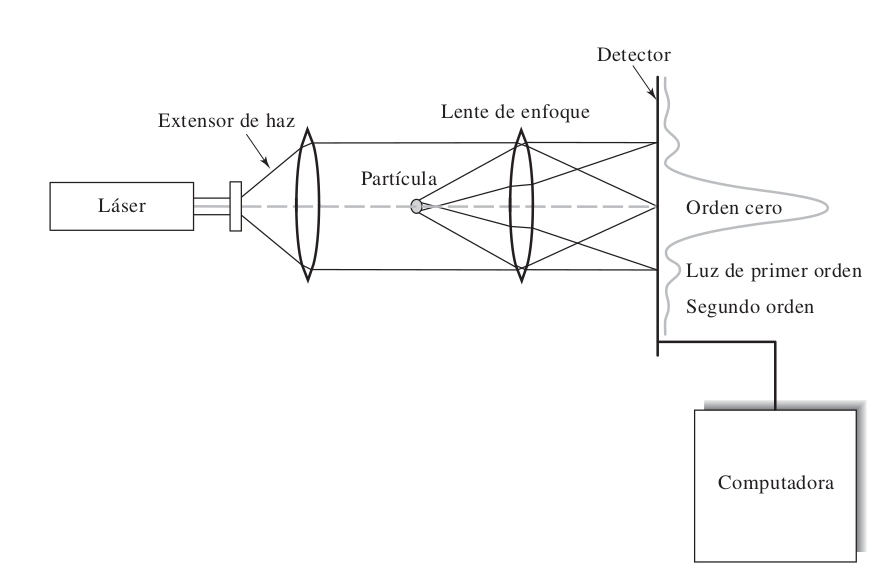
\includegraphics[width=0.65\linewidth]{Figuras/difracion_laser}
%	\caption{Esquema de un sensor de difracción láser típico, empleado para la medición de material particulado fino (fuente:Scookg 2021)}
%	\label{fig:difracionlaser}
%\end{figure}





\section{2. Identificación y análisis de los interesados}
\label{sec:interesados}
%!TEX root = DisenoProyecto_LuisGomez.tex

%\begin{consigna}{red} % este comando se debe borrar para la entrega, junto con la contraparte \end{consigna}{red} 
% 
%\textbf{Nota importante:} borrar esto y todas las consignas en color rojo antes de entregar este documento). Esto se hace eliminando el par de comandos que forman el bloque consigna, \verb!\begin{consigna}{red}! y \verb!\end{consigna}{red}! del código. 
% 
%Es inusual que una misma persona esté en más de un rol, incluso en proyectos chicos. Si se considera que una persona cumple dos o más roles, entonces solo dejarla en el rol más importante. 
%
%Por ejemplo, si una persona es Cliente pero también colabora u orienta, dejarla solo como Cliente. Si una persona es el Responsable, no debe ser colocado también como miembro del equipo.


\begin{table}[ht]
\caption{Identificación de los interesados.}
\label{tab:interesados}
\begin{tabularx}{\linewidth}{@{}|l|X|X|l|@{}}
\hline
\rowcolor[HTML]{C0C0C0} 
Rol           & Nombre y Apellido & Organización 	& Puesto 	\\ \hline
%Auspiciante   &      -             &        -      	&    -    	\\ \hline
Cliente       & \clientename      &\empclientename	& Investigadora       	\\ \hline
%Impulsor      &        -           &       -       	&    -    	\\ \hline
Responsable   & \authorname       & FIUBA        	& Alumno 	\\ \hline
%Colaboradores &       -            &       -       	&     -   	\\ \hline
Orientador    & \supname	      & \pertesupname 	& Director Trabajo final \\ \hline
%Equipo        &      -       	  &           -   	&    -   	\\ \hline
%Opositores    &       -            &        -      	&       - 	\\ \hline
Usuario final &      Comunidades afectadas  &     -         	&      -  	\\ \hline
\end{tabularx}
\end{table}

%El Director suele ser uno de los Orientadores.
%
%No dejar celdas vacías; si no hay nada que poner en una celda colocar un signo ``-''.
%
%No dejar filas vacías; si no hay nada que poner en una fila entonces eliminarla.
%
%Es deseable listar a continuación las principales características de cada interesado.
% 
%Por ejemplo:
\begin{description}
\item [Cliente:] doctora en Química Ambiental especializada en monitoreo de calidad del aire. Actualmente lidera proyectos de relevancia nacional en Chile, como Fodequip Mayor y Fodecyt, enfocados en la implementación y evaluación de sensores de bajo costo para el monitoreo ambiental. Se espera su aporte en cuanto a definir características y requerimientos necesarios para un instrumental orientado a estimar las concentraciones de MP2,5.
%	\item Auspiciante: es riguroso y exigente con la rendición de gastos. Tener mucho cuidado con esto.
%	\item Equipo: Juan Perez, suele pedir licencia porque tiene un familiar con una enfermedad. Planificar considerando esto.
\item [Orientador:] ingeniero electrónico con amplia experiencia tanto en el ámbito profesional como en la docencia. Su contribución será fundamental en el diseño de la placa electrónica que soportará el instrumental y en la optimización de la programación del microcontrolador.

\item [Usuario Final:] el usuario final está constituido principalmente por la población urbana expuesta a episodios de contaminación atmosférica relacionados con MP2,5. Estos episodios son especialmente prevalentes durante ciertos días de invierno y pueden representar un riesgo significativo para la salud de grupos vulnerables, como niños, ancianos y personas con enfermedades preexistentes.
\end{description}
%
%\end{consigna} % este comando se debe borrar para la entrega, junto con la contraparte \begin{consigna}{red}

\section{3. Propósito del proyecto}
\label{sec:proposito}
%!TEX root = DisenoProyecto_LuisGomez.tex

El propósito de este proyecto es desarrollar un equipo de medición de material particulado fino (MP2,5) que brinde una mayor precisión y exactitud que los sensores ópticos de bajo costo, mediante técnicas estadísticas de muestreo. El dispositivo también contará con características para almacenar y transmitir datos de forma remota. Se pretende elaborar una solución económica y fiable que pueda integrarse en las redes de control de calidad del aire, comúnmente gestionadas por autoridades ambientales o gobiernos locales. Con esto se espera contribuir a la mejora de la salud pública en entornos urbanos. 


%\begin{consigna}{red}
%¿Por qué se hace el proyecto? ¿Qué se quiere lograr? 
%
%Se recomienda que sea solo un párrafo que empiece diciendo ``El propósito de este proyecto es...''.
%\end{consigna}


\section{4. Alcance del proyecto}
\label{sec:alcance}
%!TEX root = DisenoProyecto_LuisGomez.tex
En este proyecto se incluyen las siguientes actividades:

\begin{enumerate}[label=\alph*)]
	\item \textbf{Diseño y desarrollo del hardware}
	\begin{itemize}
		\item Diseño y dimensionamiento del hardware acorde a los niveles de consumo eléctrico, necesidad de cómputo, almacenamiento y transmisión de datos.  
		\item Selección y adquisición los sensores ópticos de MP2,5, y el microcontrolador central, adecuado a los requerimientos de cómputo y administración del sistema.
		\item Diseño del sistema de almacenamiento de datos y del mecanismo de transmisión de información. Cada dato deberá contar con hora y fecha. Esta información debe ser proporcionada a partir de la implementación del RTC.
		\item Dimensionamiento del sistema de alimentación eléctrica acorde a los requerimientos del hardaware .
	\end{itemize}
	
	\item \textbf{Desarrollo de software}
	\begin{itemize}
		\item Programación del microprocesador para realizar cálculos y transmitir resultados.
		\item Desarrollo de algoritmos para efectuar estadísticas en tiempo real.
		\item Generación de algoritmo para el chequeo del funcionamiento de los sensores e implementación de códigos de error en caso de que alguno falle.
	\end{itemize}
	
	\item \textbf{Pruebas de calibración}
	\begin{itemize}
		\item Calibración inicial de los sensores con estaciones de monitoreo de referencia o instrumentos de referencia disponibles.
	\end{itemize}
	
	\item \textbf{Recolección de datos}
	\begin{itemize}
		\item Periodo de recolección de datos de MP2,5 para evaluar el funcionamiento y rendimiento del dispositivo.
	\end{itemize}
	
	\item \textbf{Análisis de datos}
	\begin{itemize}
		\item Evaluación de precisión y exactitud del dispositivo en comparación con los métodos ópticos tradicionales y los de referencia.
	\end{itemize}
	
	\item \textbf{Documentación}
	\begin{itemize}
		\item Generación de informes técnicos que validen el rendimiento y robustez del dispositivo.
	\end{itemize}
	
\end{enumerate}

El presente proyecto no incluye las siguientes actividades:

\begin{enumerate}[label=\alph*)]
	
	\item \textbf{Despliegue a gran escala}
	\begin{itemize}
		\item Este proyecto no incluye la fabricación en masa ni la distribución a gran escala del dispositivo.
	\end{itemize}
	
	\item \textbf{Mantenimiento prolongado}
	\begin{itemize}
		\item El mantenimiento del dispositivo más allá del periodo de pruebas no está incluido.
	\end{itemize}
	
	\item \textbf{Formación o capacitación}
	\begin{itemize}
		\item No se incluye la formación o capacitación para usuarios finales o para entidades gubernamentales.
	\end{itemize}
	
	\item \textbf{Adopción por parte de las autoridades}
	\begin{itemize}
		\item Aunque se espera que las autoridades consideren esta tecnología, su adopción oficial no está garantizada dentro del alcance de este proyecto.
	\end{itemize}
	
	\item \textbf{Investigaciones futuras}
	\begin{itemize}
		\item No se incluye el seguimiento a largo plazo de la efectividad del dispositivo en políticas públicas o investigaciones futuras.
	\end{itemize}
	
\end{enumerate}


%\begin{consigna}{red}
%¿Qué se incluye y que no se incluye en este proyecto?
%
%Se refiere al trabajo a hacer para entregar el producto o resultado especificado. 
%
%Explicitar todo lo quede comprendido dentro del alcance del proyecto.
%
%Explicitar además todo lo que no quede incluido (``El presente proyecto no incluye...'')

%\end{consigna}


\section{5. Supuestos del proyecto}
\label{sec:supuestos}
%!TEX root = DisenoProyecto_LuisGomez.tex
% SUPUESTOS 
%\begin{consigna}{red}
%``Para el desarrollo del presente proyecto se supone que: ...''
%
%\begin{itemize}
%	\item Supuesto 1
%	\item Supuesto 2...
%\end{itemize}
%
%Por ejemplo, se podrían incluir supuestos respecto a disponibilidad de tiempo y recursos humanos y materiales, sobre la factibilidad técnica de distintos aspectos del proyecto, sobre otras cuestiones que sean necesarias para el éxito del proyecto como condiciones macroeconómicas o reglamentarias.
%\end{consigna}
Mediante la implementación simultánea de tres sensores ópticos dedicados a la cuantificación de partículas finas atmosféricas (MP2,5), se espera generar conjunto de datos replicados que permitan realizar análisis estadísticos en tiempo real. Este diseño metodológico no solamente facilita la obtención de valores promedio más confiables, sino que también posibilita un proceso de validación o exclusión de observaciones anómalas que se desvíen significativamente de la media poblacional. Desde una perspectiva estadística, se espera que un mayor volumen muestral contribuirá al incremento tanto de la precisión como de la exactitud en las mediciones. Concretamente, se espera lograr una reducción en el Error Estándar de la Media (ESM) y un acercamiento más preciso al valor verdadero de la media poblacional ($\mu$), conforme a los principios del Teorema del Límite Central.

En términos de robustez del sistema, la presencia de múltiples sensores se estima que proporcione una capa adicional de confiabilidad. En caso de mal funcionamiento de algún sensor, el sistema de microcontrolador estará diseñado para detectar el problema, lo que permite la implementación de soluciones preventivas antes de una posible interrupción completa del equipo.

Finalmente, aunque estos sensores ópticos no están actualmente reconocidos por la Agencia de Protección Ambiental (EPA) como una técnica analítica estándar para la medición de MP2,5, su adopción por parte de autoridades y entidades gubernamentales ayudaría como un complemento eficaz y económico a las redes de monitoreo existentes. Esta incorporación no solo fortalecería las estrategias de monitoreo actualmente en uso, sino que también podría servir como un primer paso para establecer estaciones de monitoreo en áreas que actualmente carecen de ellas.


\subsection{Otros Supuestos}

\begin{itemize}
	
	\item \textbf{Calibración con estaciones de referencia:} se espera que los sensores puedan calibrarse utilizando estaciones de referencia EPA certificadas por instituciones con competencia.
	
	\item \textbf{Precisión de datos históricos:} se asume que los datos obtenidos durante los procesos de calibración con sistemas gravimétricos o estaciones de monitoreo existentes son precisos y representativos. Además, se espera que estos datos sean comparables a pesar de las diferencias en las frecuencias de muestreo entre las tecnologías.
	
	\item \textbf{Mantenimiento de la calibración:} una vez calibrados, se espera que los sensores mantengan su calibración durante todo el periodo de recolección de datos, sin requerir ajustes frecuentes para mantener su precisión y exactitud.
	
	\item \textbf{Estabilidad de condiciones ambientales:} se asume que las condiciones ambientales, como temperatura y humedad, no afectarán significativamente la precisión y la capacidad de medición de los sensores durante periodos prolongados.
	
	\item \textbf{Ausencia de interferencias:} se presupone que otras partículas o sustancias en el ambiente, como los aerosoles de agua, no interferirán significativamente en la medición del material particulado de interés.
	
	\item \textbf{Energía y conectividad constantes:} se espera contar con un suministro constante y fiable de energía y conectividad de datos durante la ejecución del proyecto.
	
	\item \textbf{Aceptación por parte de los interesados:} se anticipa que autoridades ambientales y otros grupos de interés estarán abiertos a considerar y, posiblemente, adoptar esta tecnología si se demuestra su eficacia.
	
	\item \textbf{Escalabilidad del sistema:}  se prevé que el sistema podrá funcionar en exteriores y escalarse para cubrir áreas geográficas más grandes o para incorporar tipos de mediciones ambientales adicionales sin cambios significativos en su arquitectura.
	
	\item \textbf{Futura conformidad regulatoria:} aunque los sensores no están actualmente estandarizados por la EPA, se espera que futuras regulaciones puedan incluir este tipo de tecnologías. Es relevante señalar que la Comunidad Económica Europea está evaluando actualmente esta posibilidad.
	
	\item \textbf{Participación comunitaria:} si los datos recolectados se utilizaran para la toma de decisiones a nivel comunitario, se espera un nivel adecuado de compromiso y participación por parte de la comunidad local.
	
	\item \textbf{Costos operativos controlables:} se estima que los costos operativos y de mantenimiento del sistema se mantendrán dentro de un rango predecible y manejable durante su vida útil.
	
\end{itemize}




\section{6. Requerimientos}
\label{sec:requerimientos}
%!TEX root = DisenoProyecto_LuisGomez.tex

%\begin{consigna}{red}
%Los requerimientos deben numerarse y de ser posible estar agruparlos por afinidad, por ejemplo:
%
%\begin{enumerate}
%	\item Requerimientos funcionales
%		\begin{enumerate}
%			\item El sistema debe...
%			\item Tal componente debe...
%			\item El usuario debe poder...
%		\end{enumerate}
%	\item Requerimientos de documentación
%		\begin{enumerate}
%			\item Requerimiento 1
%			\item Requerimiento 2 (prioridad menor)
%		\end{enumerate}
%	\item Requerimiento de testing...
%	\item Requerimientos de la interfaz...
%	\item Requerimientos interoperabilidad...
%	\item etc...
%\end{enumerate}
%
%Leyendo los requerimientos se debe poder interpretar cómo será el proyecto y su funcionalidad.
%
%Indicar claramente cuál es la prioridad entre los distintos requerimientos y si hay requerimientos opcionales. 
%
%No olvidarse de que los requerimientos incluyen a las regulaciones y normas vigentes!!!
%
%Y al escribirlos seguir las siguientes reglas:
%\begin{itemize}
%	\item Ser breve y conciso (nadie lee cosas largas). 
%	\item Ser específico: no dejar lugar a confusiones.
%	\item Expresar los requerimientos en términos que sean cuantificables y medibles.
%\end{itemize}
%
%\end{consigna}
En esta sección, se enumeran los requisitos del sistema de acuerdo a la experiencia del equipo ejecutor, características de la competencia y conversaciones con potenciales clientes. Los requisitos se clasifican en distintas categorías: requerimientos funcionales, requerimientos de hardware, requerimientos de software, requerimientos de interfaz de usuario, requerimientos de alimentación, requerimientos de evaluación y requerimientos de documentación. A cada requisito se le asigna una etiqueta de prioridad, como se muestra a continuación:
\begin{description}
	\item [\textbf{P1}]: \textbf{obligatorio}, este requisito es crucial y debe implementarse tal como se describe.
	\item [\textbf{P2}]: \textbf{importante}, es necesario implementar este requisito, aunque se pueden considerar alternativas razonables.
	\item [\textbf{P3}]: \textbf{recomendado}, su implementación es deseable, pero no esencial, y su omisión debe ser justificada.
	\item [\textbf{P4}]: \textbf{opcional}, este es un requisito que puede ser implementado a discreción del equipo de desarrollo.
\end{description}

\subsection{Requerimientos funcionales}
\begin{enumerate}[label=\alph*)]
	\item El instrumento debe incorporar al menos tres sensores dedicados a la medición de MP2,5. Prioridad: [\textbf{P1}].
	\item El dispositivo debe almacenar localmente los datos de MP2,5, ofreciendo la opción de consultar y vaciar la memoria cuando sea necesario. Prioridad: [\textbf{P1}]
	\item El sistema debe calcular automáticamente los parámetros estadísticos relevantes, como el promedio, la desviación estándar, valores mínimos y máximos, y detectar valores fuera de rango. Prioridad: [\textbf{P2}]
	\item La comunicación entre el nodo sensor y el servidor debe ser flexible, admitiendo conexiones cableadas o inalámbricas mediante protocolos como Wi-Fi (IEEE 802.11n) o LoRa. Prioridad: [\textbf{P3}]
	\item Cada instrumento debe ser identificable de manera única dentro del sistema, permitiendo garantizar una correcta asociación de los datos recolectados con el sensor. Prioridad: [\textbf{P2}]
	\item Todas las mediciones deben ser acompañadas de una estampa temporal proporcionada por un Reloj de Tiempo Real (RTC). Prioridad: [\textbf{P1}]
	\item El instrumento debe ofrecer funcionalidades de monitoreo remoto que permitan verificar su estado operativo, calibraciones y ajustes. Prioridad: [\textbf{P4}]
	\item El sistema debe ser capaz de generar y almacenar promedios temporales de las mediciones, tanto en intervalos de 60 minutos como en periodos de 24 horas. Prioridad: [\textbf{P2}]
\end{enumerate}
\subsection{Requerimientos de hardware}
\begin{enumerate}[label=\alph*)]
	\item Se usará una placa de desarrollo compatible con algún sistema de comunicación inalámbrica como Wi-Fi o LoRa. Prioridad: [\textbf{P3}]
	\item La placa de desarrollo deberá permitir conectar múltiples sensores para medir MP2,5, administrando y calculado los datos provenientes tanto de los sensores como el RTC. Prioridad: [\textbf{P1}]
	\item La comunicación entre los sensores y la placa será mediante protocolo I2C u otro similar que esté de acuerdo a las características del sensor y la placa. Prioridad: [\textbf{P1}]
	\item Rango de operación mínima de concentración del MP2,5: 0 a 500 $\mu g/m^3$ y precisión de medición: ±10\%. Prioridad: [\textbf{P2}]
\end{enumerate}
\subsection{Requerimientos de software}
\begin{enumerate}[label=\alph*)]
	\item Las variables en la que se administrarán los datos de MP2,5 serán del tipo ``constante punto flotante". Por lo tanto, el almacenamiento y las operaciones como promedio, mínimo, máximo u otro, deben también ser compatibles con este tipo de variable. Prioridad: [\textbf{P1}]
	\item Debido a que se utilizará un servidor remoto para almacenar y visualizar los datos, deberán implementarse los protocolos de comunicación acordes con el sistema de transmisión seleccionado. Prioridad: [\textbf{P4}]
	\item El programa deberá generar alarmas de funcionamiento y de fallas, que permitan al operador identificar el estado de operación del instrumento. Prioridad: [\textbf{P3}]
\end{enumerate}

\subsection{Requerimientos de interfaz de usuario}
\begin{enumerate}[label=\alph*)]
	\item El usuario debe poder acceder a los datos históricos medidos por el instrumento, ya sea leyendo la memoria incorporada en el instrumento o revisando los registros en el servidor. Prioridad: [\textbf{P2}]
	\item Debe generar alertas y notificaciones basadas en umbrales predefinidos de concentración de MP2,5. Por ejemplo, niveles críticos de medición, valores fuera de rango de medición, etc. Prioridad: [\textbf{P4}]
	\item Deberá permitir poner el sistema en modo de ahorro de energía, cuando exista una desconexión del sistema eléctrico. Prioridad: [\textbf{P3}]
\end{enumerate}
\subsection{Requerimientos de alimentación}
\begin{enumerate}[label=\alph*)]
	\item El instrumento contará con una fuente de energía compatible con la red doméstica de 220 V. Prioridad: [\textbf{P1}]
	\item El servidor y otros componentes anexos al instrumento estarán alimentados principalmente con 220 V mediante tomacorriente. Prioridad: [\textbf{P2}]
	\item A modo de seguridad, el instrumento podrá funcionar en un modo de ahorro y por tiempo reducido, mediante una batería recargable de al menos 2000 mAh. Prioridad: [\textbf{P4}]
\end{enumerate}
\subsection{Requerimientos de gabinete}
\begin{enumerate}[label=\alph*)]
	\item Los componentes del instrumento deben estar dispuestos en un gabinete individual de material plástico, con acceso a alimentación eléctrica y la entrada y salida de aire hacia y desde el censor de MP2,5. Prioridad: [\textbf{P1}]
	\item El gabinete debe ser estanco con clasificación acorde a IP65 o superior. Es decir, el gabinete debe ser adecuado para su uso en exteriores, con exposición al polvo y al agua en forma de lluvia. Prioridad: [\textbf{P2}]
	\item Facilidades para que el equipo pueda ser montado sobre postes, paredes o techos. [\textbf{P3}]
\end{enumerate}
\subsection{Requerimientos de evaluación}
\begin{enumerate}[label=\alph*)]
	\item Se debe probar el sistema en diversas condiciones atmosféricas, como humedad, temperatura, lluvias, etc. Prioridad:[\textbf{P2}]
	\item La conexión inalámbrica debe tener un área de cobertura mínima de 0,2 km. Prioridad:[\textbf{P4}]
	\item Se deben realizar pruebas de calibración con censores certificados, antes de la implementación completa. Prioridad: [\textbf{P1}]
\end{enumerate}
\subsection{Requerimientos de documentación}
\begin{enumerate}[label=\alph*)]
	\item Elaborar un manual con las características principales del instrumento, mantenimiento y sus limitaciones. Prioridad:[\textbf{P1}]
	\item La generación de tablas con posibles fallas, códigos de error y soluciones. Prioridad:[\textbf{P3}]
	\item Esquemáticos con la distribución de componentes, conexiones y alimentación eléctrica del instrumento. Prioridad: [\textbf{P1}]
\end{enumerate}


\section{7. Historias de usuarios (\textit{Product backlog})}
\label{sec:backlog}
%!TEX root = DisenoProyecto_LuisGomez.tex
%\begin{consigna}{red}
%Descripción: En esta sección se deben incluir las historias de usuarios y su ponderación (\textit{history points}). Recordar que las historias de usuarios son descripciones cortas y simples de una característica contada desde la perspectiva de la persona que desea la nueva capacidad, generalmente un usuario o cliente del sistema. La ponderación es un número entero que representa el tamaño de la historia comparada con otras historias de similar tipo.
%
%El formato propuesto es: "como [rol] quiero [tal cosa] para [tal otra cosa]."
%
%Se debe indicar explícitamente el criterio para calcular los \textit{story points} de cada historia
%\end{consigna}


A continuación, se describen diversas historias de usuario junto con su correspondiente ponderación de esfuerzo relativo o \textit{story points (SP)}. Para la ponderación de la historia utilizamos la fórmula:

\[
\text{SP} = \text{Fibo}(PtCarga + 1.5 \times PtCompl + 2 \times PtIncert)
\]

donde:
\begin{itemize}
	\item \textbf{SP}: Story points
	\item \textbf{Fibo}: Función que asigna el número de Fibonacci más cercano al argumento.
	\item \textbf{PtCarga}: Puntaje por carga de trabajo (1 a 5).
	\item \textbf{PtCompl}: Puntaje por complejidad (1 a 5).
	\item \textbf{PtIncert}: Puntaje por incertidumbre (1 a 5).
\end{itemize}

Notar que los puntajes son multiplicados por factores de ponderación antes de ser sumados.

\subsection{Historia de usuario 1: monitoreo de concentraciones}
``Como usuario quiero poder ver las concentraciones horarias y diarias de MP2,5 que registra el sensor.''
\begin{itemize}
	\item PtCarga = 2
	\item PtCompl = 1
	\item PtIncert = 1
	\item [SP = 8]
\end{itemize}

\subsection{Historia de administrador 1: registro funcionamiento de sensores}
``Como administrador quiero que los sensores puedan generar una señal de alerta cuando uno de ellos comienza a fallar o deja de registrar.''
\begin{itemize}
	\item PtCarga = 3
	\item PtCompl = 4
	\item PtIncert = 2
	\item [SP = 13]
\end{itemize}

\subsection{Historia de usuario 2: alarmas por concentración}
``Como usuario quiero que el instrumento me indique cuando existen valores críticos de concentración, que puedan ser riesgosos para la salud de la población.''
\begin{itemize}
	\item PtCarga = 4
	\item PtCompl = 3
	\item PtIncert = 3
	\item [SP = 21]
\end{itemize}

\subsection{Historia de administrador 2: precisión de la concentración}
``Como administrador quiero conocer la precisión de los valores que estoy registrando.''
\begin{itemize}
	\item PtCarga = 4
	\item PtCompl = 3
	\item PtIncert = 3
	\item [SP = 21]
\end{itemize}

% ... Puedes seguir añadiendo más historias de usuario



% Añadir más historias de usuario según sea necesario.



\section{8. Entregables principales del proyecto}
\label{sec:entregables}
%!TEX root = DisenoProyecto_LuisGomez.tex
%\begin{consigna}{red}
%
Los entregables del proyecto  con sus fechas propuestas son:

\begin{itemize}
	\item Escrito con proyecto de tesis (13 octubre 2023)
	\item Prototipo funcional (6 de marzo del 2024)
	\item Manual de uso (8 de mayo del 2024)
	\item Informe final (22 de mayo del 2024)
	\item Diapositivas con presentación del instrumento (22 de mayo del 2024)
\end{itemize}
%
%\end{consigna}

\section{9. Desglose del trabajo en tareas}
\label{sec:wbs}
%!TEX root = DisenoProyecto_LuisGomez.tex
%\begin{consigna}{red}
%El WBS debe tener relación directa o indirecta con los requerimientos.  Son todas las actividades que se harán en el proyecto para dar cumplimiento a los requerimientos. Se recomienda mostrar el WBS mediante una lista indexada:
%
%\begin{enumerate}
%\item Grupo de tareas 1
%	\begin{enumerate}
%	\item Tarea 1 (tantas h)
%	\item Tarea 2 (tantas hs)
%	\item Tarea 3 (tantas h)
%	\end{enumerate}
%\item Grupo de tareas 2
%	\begin{enumerate}
%	\item Tarea 1 (tantas h)
%	\item Tarea 2 (tantas h)
%	\item Tarea 3 (tantas h)
%	\end{enumerate}
%\item Grupo de tareas 3
%	\begin{enumerate}
%	\item Tarea 1 (tantas h)
%	\item Tarea 2 (tantas h)
%	\item Tarea 3 (tantas h)
%	\item Tarea 4 (tantas h)
%	\item Tarea 5 (tantas h)
%	\end{enumerate}
%\end{enumerate}
%
%Cantidad total de horas: (tantas h)
%
%Se recomienda que no haya ninguna tarea que lleve más de 40 h. 
%
%\end{consigna}


\label{sec:wbs}

En el siguiente apartado, se llevará a cabo un desglose detallado de las actividades y tareas propuestas para la ejecución del proyecto de tesis de la Carrera. Cada actividad será identificada utilizando la numeración del work breakdown structure (WBS) para asegurar una organización y seguimiento efectivos. Adicionalmente, se especificarán tanto los tiempos parciales como los tiempos totales requeridos para cada tarea, expresados en formato de hora.

Esta estructuración tiene como objetivo proporcionar una visión completa y ordenada del proyecto, permitiendo una asignación y gestión eficiente de los recursos temporales. Como se muestra a continuación, se estima el trabajo total del proyecto de tesis en unas 730 horas cronológicas, divididas en ocho secciones.



\begin{enumerate}
	\item\textbf{ Gestión del proyecto (100 h)}
	\begin{enumerate}
		\item Generación de requerimientos (20 h)
		\item Planificación del proyecto (40 h)
		\item Planificación de entregables (10 h)
		\item Revisión y ajustes de planificación (30 h)
	\end{enumerate}
	
	\item\textbf{Diseño general (60 h)}
	\begin{enumerate}
		\item Ajuste al diseño conceptual (10 h)
		\item Diagramas de flujo y arquitectura (20 h)
		\item Revisión y pruebas de diseño (30 h)
	\end{enumerate}
	
	\item \textbf{Construcción del hardware (120 h)}
	\begin{enumerate}
		\item Selección de componentes (20 h)
		\item Diseño de circuitos (40 h)
		\item Montaje y soldadura (30 h)
		\item Pruebas iniciales (30 h)
	\end{enumerate}
	
	\item \textbf{Diseño del firmware (110 h)}
	\begin{enumerate}
		\item Diseño de la arquitectura del software (20 h)
		\item Implementación de la medición de MP2,5 (30 h)
		\item Implementación de almacenamiento y comunicación (30 h)
		\item Implementación de funciones auxiliares (30 h)
	\end{enumerate}
	
	\item \textbf{Realización de pruebas (80 h)}
	\begin{enumerate}
		\item Diseño de casos de prueba (20 h)
		\item Ejecución de pruebas (40 h)
		\item Análisis de resultados (20 h)
	\end{enumerate}
	
	\item \textbf{Ajustes finales instrumento (40 h)}
	\begin{enumerate}
		\item Depuración de errores (20 h)
		\item Ajustes de performance (20 h)
	\end{enumerate}
	
	\item \textbf{Escritura de memoria y manuales (180 h)}
	\begin{enumerate}
		\item Marco teórico (40 h)
		\item Metodología (30 h)
		\item Implementación (20 h)
		\item Resultados y conclusiones (20 h)
		\item Introducción, resumen y otros (30 h)
		\item Manual de usuario (20 h)
		\item Manual técnico (20 h)
	\end{enumerate}
	
	\item \textbf{Entregas del trabajo final y cierre (40 h)}
	\begin{enumerate}
		\item Proceso de cierre (20 h)
		\item Entrega y presentación del trabajo final (20 h)
	\end{enumerate}
\end{enumerate}


Cantidad total de horas: 730 hs




\newpage
\section{10. Diagrama de Activity On Node}
\label{sec:AoN}
%!TEX root = DisenoProyecto_LuisGomez.tex
%%!TEX root = DisenoProyecto_LuisGomez.tex
%%!TEX root = DisenoProyecto_LuisGomez.tex
%\input{10_Diagrama_Actividades.tex}

%\begin{consigna}{red}
%Armar el AoN a partir del WBS definido en la etapa anterior. 
%
%%La figura \ref{fig:AoN} fue elaborada con el paquete latex tikz y pueden consultar la siguiente referencia \textit{online}:
%
%%\url{https://www.overleaf.com/learn/latex/LaTeX_Graphics_using_TikZ:_A_Tutorial_for_Beginners_(Part_3)\%E2\%80\%94Creating_Flowcharts}
%
%\end{consigna}

%\begin{figure}[htpb]
%\centering 
%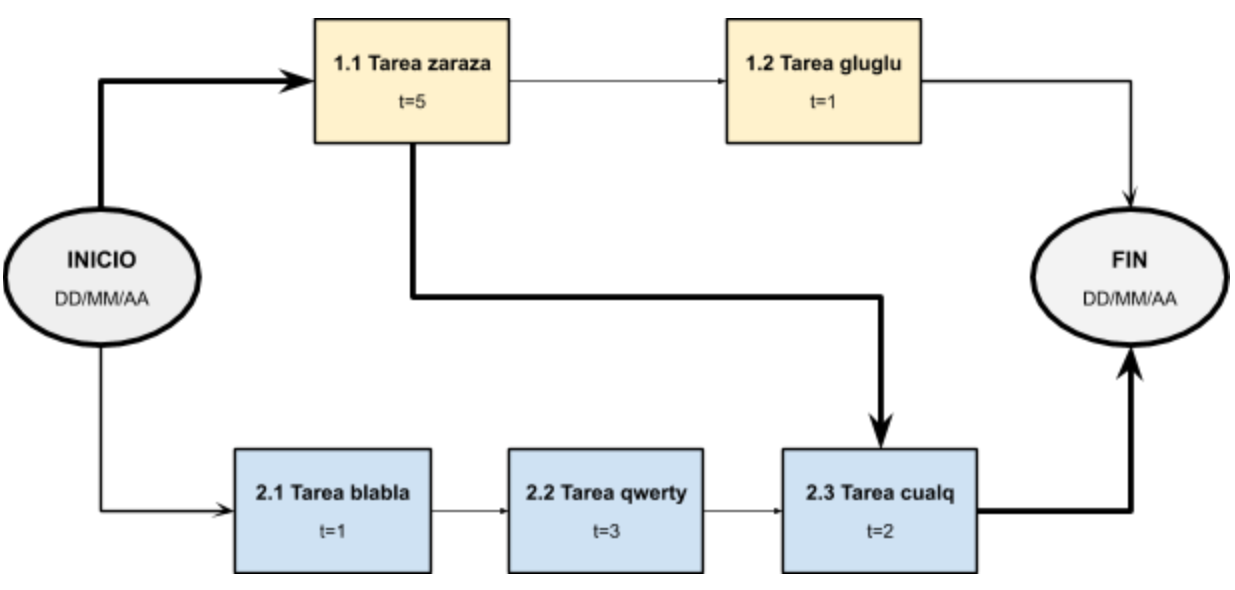
\includegraphics[width=.8\textwidth]{./Figuras/AoN.png}
%\caption{Diagrama de \textit{Activity on Node}.}
%\label{fig:AoN}
%\end{figure}
%
%Indicar claramente en qué unidades están expresados los tiempos.
%De ser necesario indicar los caminos semicríticos y analizar sus tiempos mediante un cuadro.
%Es recomendable usar colores y un cuadro indicativo describiendo qué representa cada color, como se muestra en el siguiente ejemplo:

El diagrama de flujo de la figura \ref{fig:diagrama}, se presenta una estructura general para la ejecución del proyecto de tesis. Comenzando con la gestión del proyecto, el esquema traza una ruta cronológica que incluye diseño, construcción de hardware y programación de firmware, los cuales ocurren de manera concurrente. Estas fases convergen en una etapa de pruebas, seguida de ajustes finales y la generación de documentación académica. Finalmente, el proyecto culmina con la entrega del trabajo final. Notar que cada una de las celdas contiene el tiempo estimado de las actividades y el tiempo acumulado general, con el formato:  \textbf{\textit{``tiempo bloque actividades''  / ``tiempo total acumulado"}} en horas.


\begin{figure}[!hbp]
	
	\centering
	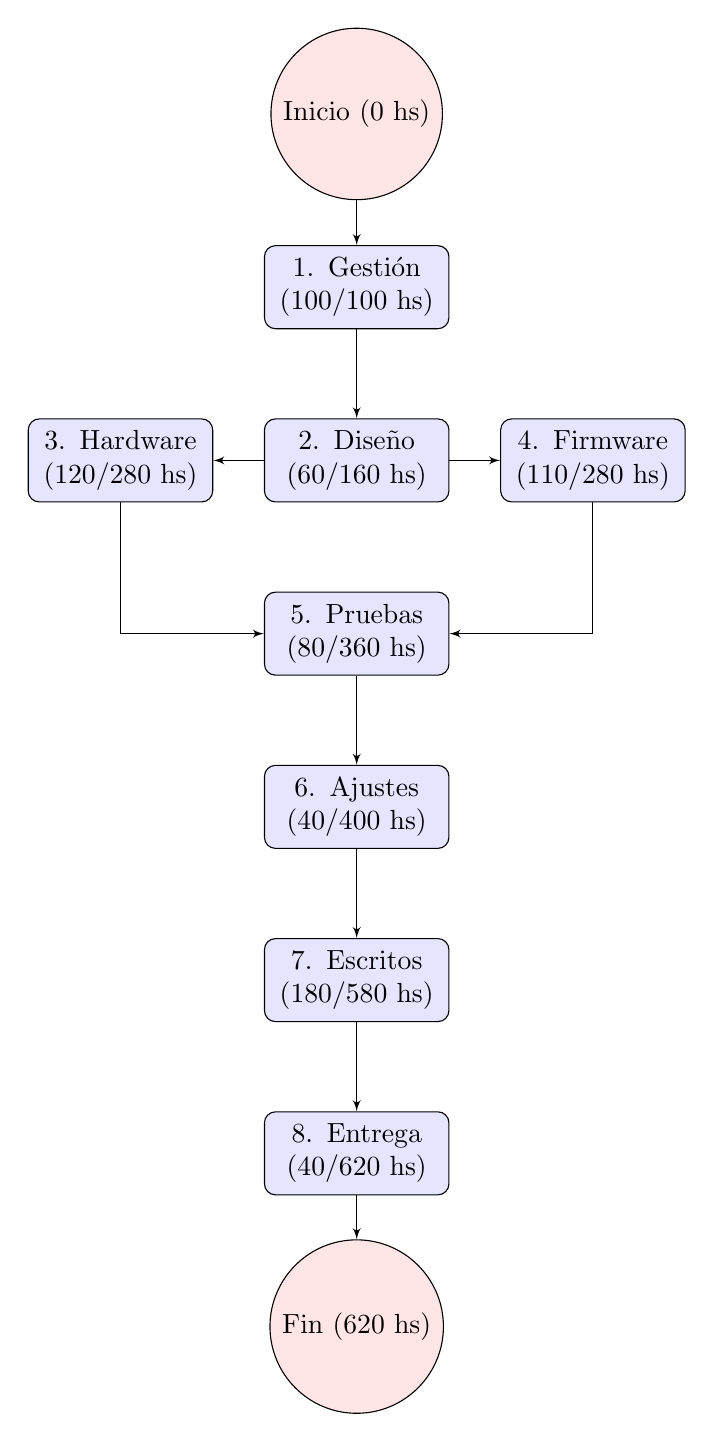
\begin{tikzpicture}[node distance=2.2cm]
	
	\tikzstyle{block} = [rectangle, draw, fill=blue!10, text width=6em, text centered, rounded corners, minimum height=3em]
	\tikzstyle{line} = [draw, -latex']
	\tikzstyle{circleblock} = [circle, draw, fill=red!10, text centered, minimum size=3em]
	
	\node [circleblock] (init) {Inicio (0 hs)};
	\node [block, below of=init]              	(1) {1. Gestión (100/100 hs)};
	\node [block, below of=1]                  	(2) {2. Diseño (60/160 hs)};
	\node [block, left of=2, node distance=3cm]	(3) {3. Hardware (120/280 hs)};
	\node [block, right of=2, node distance=3cm](4) {4. Firmware (110/280 hs)};
	\node [block, below of=2]                  	(5) {5. Pruebas (80/360 hs)};
	\node [block, below of=5]                  	(6) {6. Ajustes (40/400 hs)};
	\node [block, below of=6]                 	(7) {7. Escritos (180/580 hs)};
	\node [block, below of=7] 					(8) {8. Entrega (40/620 hs)};
	\node [circleblock, below of=8]             (fin) {Fin (620 hs)};
	
	\path [line] (init) -- 	(1);
	\path [line] (1) 	-- 	(2);
	\path [line] (2) 	-- 	(3);
	\path [line] (2) 	-- 	(4);
	\path [line] (4) 	|- 	(5);
	\path [line] (3) 	|- 	(5);
	\path [line] (5) 	-- 	(6);
	\path [line] (6) 	-- 	(7);
	\path [line] (7) 	-- 	(8);
	\path [line] (8) 	-- 	(fin);
	
	
	\end{tikzpicture}
	\caption{Diagrama de flujo para la gestión del proyecto}
	\label{fig:diagrama}
\end{figure}






%\begin{consigna}{red}
%Armar el AoN a partir del WBS definido en la etapa anterior. 
%
%%La figura \ref{fig:AoN} fue elaborada con el paquete latex tikz y pueden consultar la siguiente referencia \textit{online}:
%
%%\url{https://www.overleaf.com/learn/latex/LaTeX_Graphics_using_TikZ:_A_Tutorial_for_Beginners_(Part_3)\%E2\%80\%94Creating_Flowcharts}
%
%\end{consigna}

%\begin{figure}[htpb]
%\centering 
%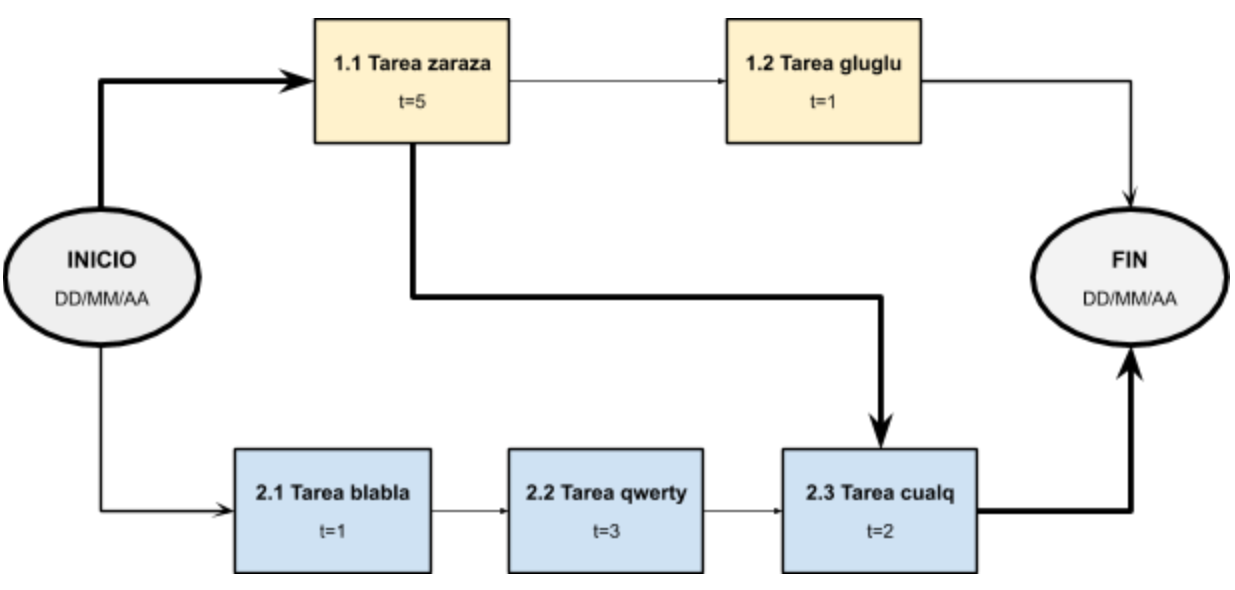
\includegraphics[width=.8\textwidth]{./Figuras/AoN.png}
%\caption{Diagrama de \textit{Activity on Node}.}
%\label{fig:AoN}
%\end{figure}
%
%Indicar claramente en qué unidades están expresados los tiempos.
%De ser necesario indicar los caminos semicríticos y analizar sus tiempos mediante un cuadro.
%Es recomendable usar colores y un cuadro indicativo describiendo qué representa cada color, como se muestra en el siguiente ejemplo:

El diagrama de flujo de la figura \ref{fig:diagrama}, se presenta una estructura general para la ejecución del proyecto de tesis. Comenzando con la gestión del proyecto, el esquema traza una ruta cronológica que incluye diseño, construcción de hardware y programación de firmware, los cuales ocurren de manera concurrente. Estas fases convergen en una etapa de pruebas, seguida de ajustes finales y la generación de documentación académica. Finalmente, el proyecto culmina con la entrega del trabajo final. Notar que cada una de las celdas contiene el tiempo estimado de las actividades y el tiempo acumulado general, con el formato:  \textbf{\textit{``tiempo bloque actividades''  / ``tiempo total acumulado"}} en horas.


\begin{figure}[!hbp]
	
	\centering
	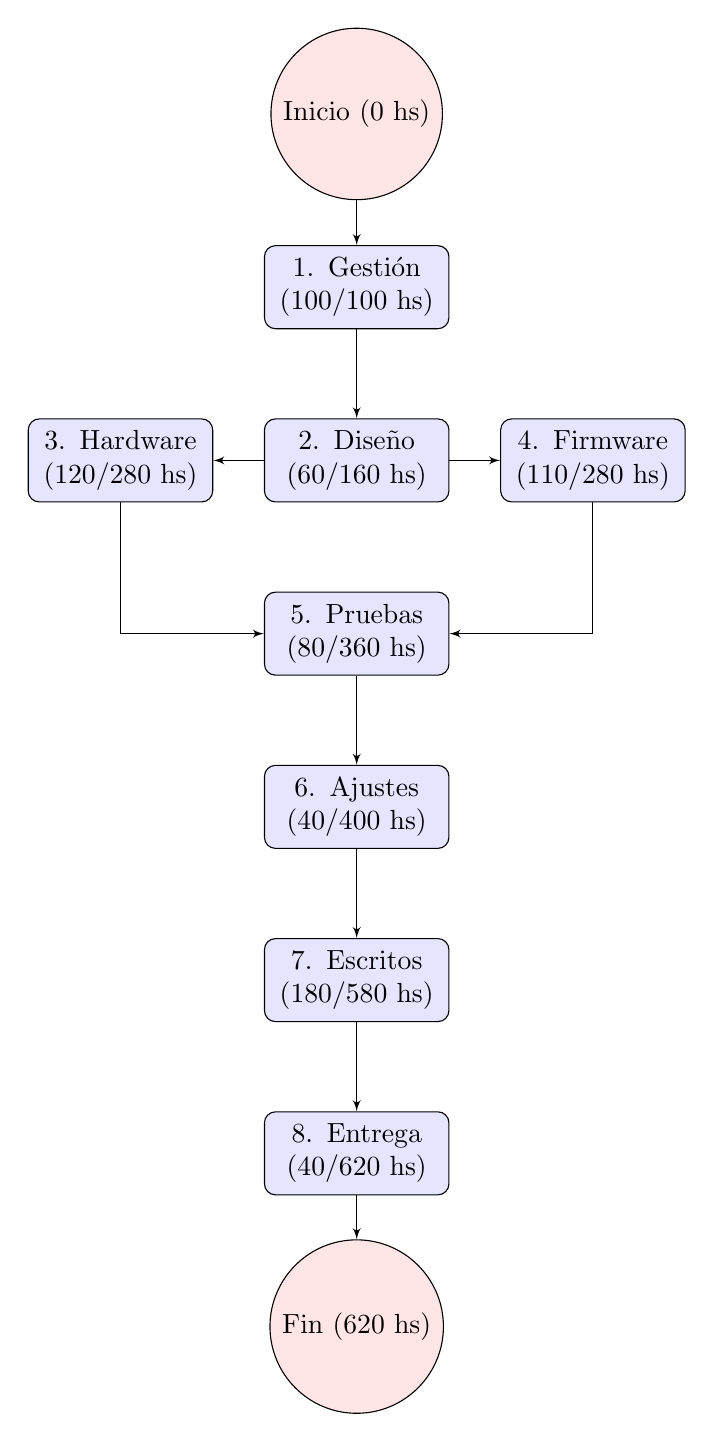
\begin{tikzpicture}[node distance=2.2cm]
	
	\tikzstyle{block} = [rectangle, draw, fill=blue!10, text width=6em, text centered, rounded corners, minimum height=3em]
	\tikzstyle{line} = [draw, -latex']
	\tikzstyle{circleblock} = [circle, draw, fill=red!10, text centered, minimum size=3em]
	
	\node [circleblock] (init) {Inicio (0 hs)};
	\node [block, below of=init]              	(1) {1. Gestión (100/100 hs)};
	\node [block, below of=1]                  	(2) {2. Diseño (60/160 hs)};
	\node [block, left of=2, node distance=3cm]	(3) {3. Hardware (120/280 hs)};
	\node [block, right of=2, node distance=3cm](4) {4. Firmware (110/280 hs)};
	\node [block, below of=2]                  	(5) {5. Pruebas (80/360 hs)};
	\node [block, below of=5]                  	(6) {6. Ajustes (40/400 hs)};
	\node [block, below of=6]                 	(7) {7. Escritos (180/580 hs)};
	\node [block, below of=7] 					(8) {8. Entrega (40/620 hs)};
	\node [circleblock, below of=8]             (fin) {Fin (620 hs)};
	
	\path [line] (init) -- 	(1);
	\path [line] (1) 	-- 	(2);
	\path [line] (2) 	-- 	(3);
	\path [line] (2) 	-- 	(4);
	\path [line] (4) 	|- 	(5);
	\path [line] (3) 	|- 	(5);
	\path [line] (5) 	-- 	(6);
	\path [line] (6) 	-- 	(7);
	\path [line] (7) 	-- 	(8);
	\path [line] (8) 	-- 	(fin);
	
	
	\end{tikzpicture}
	\caption{Diagrama de flujo para la gestión del proyecto}
	\label{fig:diagrama}
\end{figure}






%\begin{consigna}{red}
%Armar el AoN a partir del WBS definido en la etapa anterior. 
%
%%La figura \ref{fig:AoN} fue elaborada con el paquete latex tikz y pueden consultar la siguiente referencia \textit{online}:
%
%%\url{https://www.overleaf.com/learn/latex/LaTeX_Graphics_using_TikZ:_A_Tutorial_for_Beginners_(Part_3)\%E2\%80\%94Creating_Flowcharts}
%
%\end{consigna}

%\begin{figure}[htpb]
%\centering 
%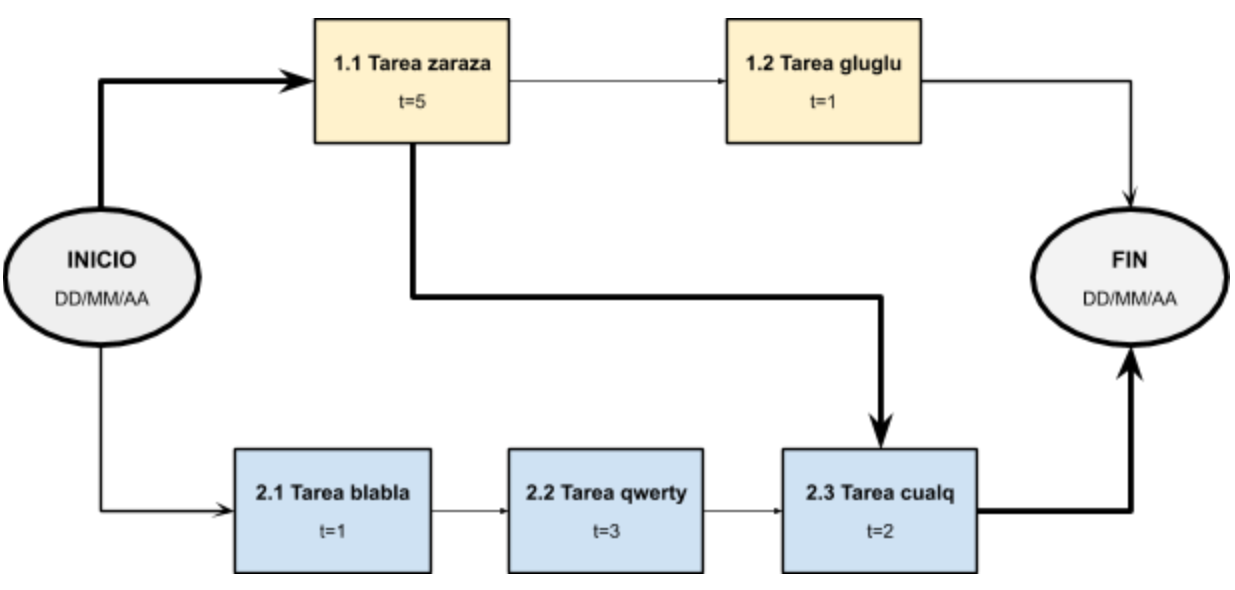
\includegraphics[width=.8\textwidth]{./Figuras/AoN.png}
%\caption{Diagrama de \textit{Activity on Node}.}
%\label{fig:AoN}
%\end{figure}
%
%Indicar claramente en qué unidades están expresados los tiempos.
%De ser necesario indicar los caminos semicríticos y analizar sus tiempos mediante un cuadro.
%Es recomendable usar colores y un cuadro indicativo describiendo qué representa cada color, como se muestra en el siguiente ejemplo:

El diagrama de flujo de la figura \ref{fig:diagrama}, se presenta una estructura general para la ejecución del proyecto de tesis. Comenzando con la gestión del proyecto, el esquema traza una ruta cronológica que incluye diseño, construcción de hardware y programación de firmware, los cuales ocurren de manera concurrente. Estas fases convergen en una etapa de pruebas, seguida de ajustes finales y la generación de documentación académica. Finalmente, el proyecto culmina con la entrega del trabajo final. Notar que cada una de las celdas contiene el tiempo estimado de las actividades y el tiempo acumulado general, con el formato:  \textbf{\textit{``tiempo bloque actividades''  / ``tiempo total acumulado"}} en horas.


\begin{figure}[!hbp]
	
	\centering
	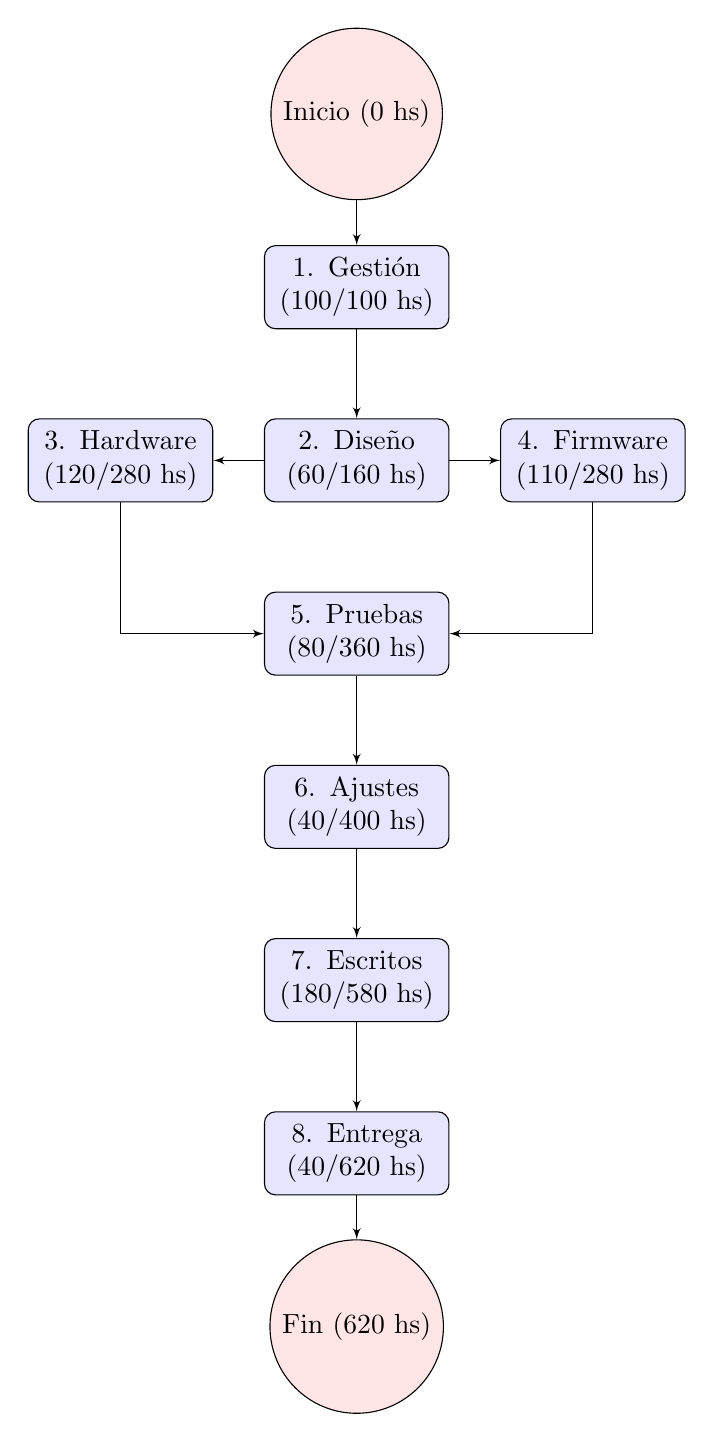
\begin{tikzpicture}[node distance=2.2cm]
	
	\tikzstyle{block} = [rectangle, draw, fill=blue!10, text width=6em, text centered, rounded corners, minimum height=3em]
	\tikzstyle{line} = [draw, -latex']
	\tikzstyle{circleblock} = [circle, draw, fill=red!10, text centered, minimum size=3em]
	
	\node [circleblock] (init) {Inicio (0 hs)};
	\node [block, below of=init]              	(1) {1. Gestión (100/100 hs)};
	\node [block, below of=1]                  	(2) {2. Diseño (60/160 hs)};
	\node [block, left of=2, node distance=3cm]	(3) {3. Hardware (120/280 hs)};
	\node [block, right of=2, node distance=3cm](4) {4. Firmware (110/280 hs)};
	\node [block, below of=2]                  	(5) {5. Pruebas (80/360 hs)};
	\node [block, below of=5]                  	(6) {6. Ajustes (40/400 hs)};
	\node [block, below of=6]                 	(7) {7. Escritos (180/580 hs)};
	\node [block, below of=7] 					(8) {8. Entrega (40/620 hs)};
	\node [circleblock, below of=8]             (fin) {Fin (620 hs)};
	
	\path [line] (init) -- 	(1);
	\path [line] (1) 	-- 	(2);
	\path [line] (2) 	-- 	(3);
	\path [line] (2) 	-- 	(4);
	\path [line] (4) 	|- 	(5);
	\path [line] (3) 	|- 	(5);
	\path [line] (5) 	-- 	(6);
	\path [line] (6) 	-- 	(7);
	\path [line] (7) 	-- 	(8);
	\path [line] (8) 	-- 	(fin);
	
	
	\end{tikzpicture}
	\caption{Diagrama de flujo para la gestión del proyecto}
	\label{fig:diagrama}
\end{figure}







\section{11. Diagrama de Gantt}
\label{sec:gantt}
%\begin{landscape}
%!TEX root = DisenoProyecto_LuisGomez.tex

%%!TEX root = DisenoProyecto_LuisGomez.tex

%%!TEX root = DisenoProyecto_LuisGomez.tex

%\input{11_Diagrama_Gantt.tex}

%\begin{consigna}{red}
%
%Existen muchos programas y recursos \textit{online} para hacer diagramas de Gantt, entre los cuales destacamos:
%
%\begin{itemize}
%\item Planner
%\item GanttProject
%\item Trello + \textit{plugins}. En el siguiente link hay un tutorial oficial: \\ \url{https://blog.trello.com/es/diagrama-de-gantt-de-un-proyecto}
%\item Creately, herramienta online colaborativa. \\\url{https://creately.com/diagram/example/ieb3p3ml/LaTeX}
%\item Se puede hacer en latex con el paquete \textit{pgfgantt}\\ \url{http://ctan.dcc.uchile.cl/graphics/pgf/contrib/pgfgantt/pgfgantt.pdf}
%\end{itemize}
%
%Pegar acá una captura de pantalla del diagrama de Gantt, cuidando que la letra sea suficientemente grande como para ser legible. 
%Si el diagrama queda demasiado ancho, se puede pegar primero la ``tabla'' del Gantt y luego pegar la parte del diagrama de barras del diagrama de Gantt.
%
%Configurar el software para que en la parte de la tabla muestre los códigos del EDT (WBS).\\
%Configurar el software para que al lado de cada barra muestre el nombre de cada tarea.\\
%Revisar que la fecha de finalización coincida con lo indicado en el Acta Constitutiva.
%
%En la figura \ref{fig:gantt}, se muestra un ejemplo de diagrama de Gantt realizado con el paquete de \textit{pgfgantt}. En la plantilla pueden ver el código que lo genera y usarlo de base para construir el propio.
%
%\begin{figure}[htbp]
%\begin{center}
%\begin{ganttchart}{1}{12}
%  \gantttitle{2020}{12} \\
%  \gantttitlelist{1,...,12}{1} \\
%  \ganttgroup{Group 1}{1}{7} \\
%  \ganttbar{Task 1}{1}{2} \\
%  \ganttlinkedbar{Task 2}{3}{7} \ganttnewline
%  \ganttmilestone{Milestone o hito}{7} \ganttnewline
%  \ganttbar{Final Task}{8}{12}
%  \ganttlink{elem2}{elem3}
%  \ganttlink{elem3}{elem4}
%\end{ganttchart}
%\end{center}
%\caption{Diagrama de Gantt de ejemplo}
%\label{fig:gantt}
%\end{figure}
%
%
%\begin{landscape}
%\begin{figure}[htpb]
%\centering 
%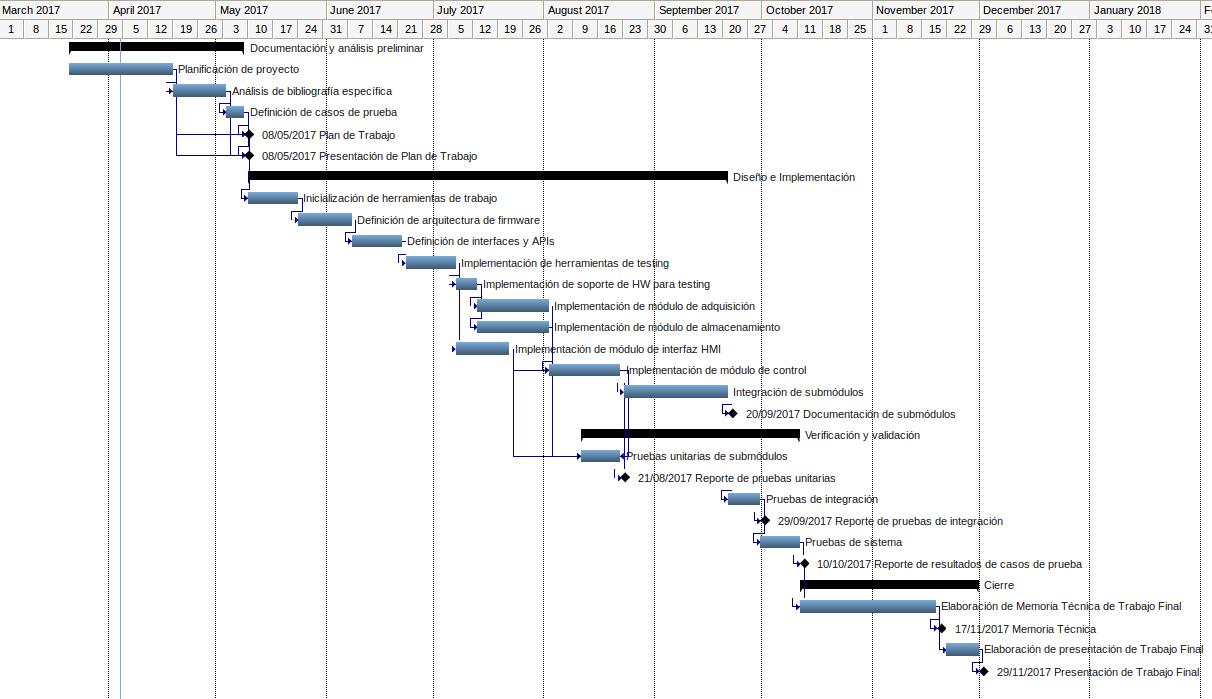
\includegraphics[height=.85\textheight]{./Figuras/Gantt-2.png}
%\caption{Ejemplo de diagrama de Gantt rotado}
%\label{fig:diagGantt}
%\end{figure}
%
%\end{landscape}
%
%\end{consigna}

%\begin{landscape}
\rotatebox{90}{%
\begin{ganttchart}[
	hgrid,
    vgrid={*4{dotted}, *3{red!50}}, %	vgrid,
	x unit=0.12cm,
	y unit chart=0.7cm,
	time slot format=isodate,
	time slot unit=day,
	bar/.append style={fill=blue!30},
	group/.append style={fill=blue!50},
	%link/.style={->, thick}
	]{2023-09-11}{2024-01-24}
	
	\gantttitlecalendar{year, month} \\
			\ganttmilestone{0. Acta de Constitución}{2023-09-11}\\
		\ganttgroup{1 Gestión del Proyecto}{2023-09-11}{2023-10-13} \\
		\ganttbar[name=11]{1.1 Generación de requerimientos}{2023-09-11}{2023-09-15} \\
		\ganttbar[name=12]{1.2 Planificación del proyecto}{2023-09-18}{2023-09-29} \\
		\ganttbar{1.3 Planificación de entregables}{2023-10-02}{2023-10-04} \\
		\ganttbar{1.4 Revisión y ajustes}{2023-10-04}{2023-10-13} \\
			\ganttmilestone{1.5 Proyecto de tesis}{2023-10-13} \\
	
	\ganttgroup{2 Diseño General}{2023-10-16}{2023-11-03} \\
		\ganttbar{2.1 Ajuste al diseño conceptual}{2023-10-16}{2023-10-18} \\
		\ganttbar{2.2 Diagramas de flujo}{2023-10-18}{2023-10-25} \\
		\ganttbar{2.3 Revisión y ajustes de diseño}{2023-10-25}{2023-11-03} \\
	
	\ganttgroup{3 Construcción del hardware}{2023-11-06}{2023-12-15} \\
		\ganttbar{3.1 Selección de componentes}{2023-11-06}{2023-11-10} \\
		\ganttbar{3.2 Diseño de circuitos}{2023-11-13}{2023-11-24} \\
		\ganttbar{3.3 Montaje y soldadura}{2023-11-27}{2023-12-06} \\
		\ganttbar{3.4 Pruebas iniciales}{2023-12-06}{2023-12-15} \\
	
	\ganttgroup{4 Diseño del firmware}{2023-12-18}{2024-01-24} \\
		\ganttbar{4.1 Diseño de arquitectura}{2023-12-18}{2023-12-22} \\
		\ganttbar{4.2 Implementación de MP2,5}{2023-12-25}{2024-01-03} \\
		\ganttbar{4.3 Almacenamiento y comunicación}{2024-01-03}{2024-01-12} \\
		\ganttbar{4.4 Funciones auxiliares}{2024-01-15}{2024-01-24} 
	
	\ganttlink[]{11}{12}
	
\end{ganttchart}
}
\newpage
\rotatebox{90}{%
\begin{ganttchart}[
	hgrid,
%vgrid,
 vgrid={*4{dotted}, *3{red!50}}, %	vgrid,
x unit=0.14cm,
y unit chart=0.7cm,
time slot format=isodate,
time slot unit=day,
bar/.append style={fill=blue!30},
group/.append style={fill=blue!50},
bar/.append style={fill=blue!30, bar label node/.append style={above=3pt}},
%include title in canvas=false,
%inline,
milestone inline label node/.append style={left=5mm}
%link/.style={->, thick}
%link label font=\small\bfseries\color{purple}
link/.style={|-to, line width=0.5pt, blue},
    bar inline label node/.style={
	anchor=east,
	xshift=+4.5cm,
	yshift=0.4cm,
}
]{2024-01-22}{2024-05-28}
	
	\gantttitlecalendar{year, month} \\
	
	\ganttgroup{5 Realización de pruebas}{2024-01-24}{2024-02-21} \\
		\ganttbar[name=51]{5.1 Diseño de casos de prueba}{2024-01-24}{2024-01-31} \\
		\ganttbar[name=52]{5.2 Ejecución de pruebas}{2024-01-31}{2024-02-14} \\
		\ganttbar[name=53]{5.3 Análisis de resultados}{2024-02-14}{2024-02-21} \\
		
	\ganttgroup{6 Ajustes finales}{2024-02-21}{2024-03-06} \\
		\ganttbar[name=61]{6.1 Depuración de errores}{2024-02-21}{2024-02-28} \\
		\ganttbar{6.2 Ajustes de performance}{2024-02-28}{2024-03-06} \\
			\ganttmilestone{6.3 Prototipo funcional}{2024-03-06} \\
		
	\ganttgroup{7 Generación escrito y manuales}{2024-03-06}{2024-05-08} \\
		\ganttbar{7.1 Marco teórico}{2024-03-06}{2024-03-20} \\
		\ganttbar{7.2 Metodología}{2024-03-20}{2024-03-27} \\
		\ganttbar{7.3 Implementación}{2024-03-27}{2024-04-03} \\
		\ganttbar{7.4 Resultados y conclusiones}{2024-04-03}{2024-04-10} \\
		\ganttbar{7.5 Introducción, resumen y otros}{2024-04-10}{2024-04-19} \\
		\ganttbar{7.6 Manual de usuario}{2024-04-22}{2024-04-26} \\
		\ganttbar{7.7 Manual técnico}{2024-04-29}{2024-05-08} \\
			\ganttmilestone{7.8 Manual técnico}{2024-05-08} \\
	
	\ganttgroup{8 Entregas del trabajo final}{2024-05-08}{2024-05-22} \\
		\ganttbar{8.1 Preparación de la presentación}{2024-05-08}{2024-05-22} \\
		\ganttbar{8.2 Presentación del trabajo final}{2024-05-22}{2024-05-22} \\
			\ganttmilestone{8.3 Informe final y presentación}{2024-05-22}
	
	\ganttlink[]{51}{52}
	\ganttlink[]{52}{53}
	\ganttlink[]{53}{61}

\end{ganttchart}
%\end{landscape}
}


% TODO: \usepackage{graphicx} required

%\includegraphics[width=0.9\textwidth, angle=270]{../planner/salida}





%\begin{consigna}{red}
%
%Existen muchos programas y recursos \textit{online} para hacer diagramas de Gantt, entre los cuales destacamos:
%
%\begin{itemize}
%\item Planner
%\item GanttProject
%\item Trello + \textit{plugins}. En el siguiente link hay un tutorial oficial: \\ \url{https://blog.trello.com/es/diagrama-de-gantt-de-un-proyecto}
%\item Creately, herramienta online colaborativa. \\\url{https://creately.com/diagram/example/ieb3p3ml/LaTeX}
%\item Se puede hacer en latex con el paquete \textit{pgfgantt}\\ \url{http://ctan.dcc.uchile.cl/graphics/pgf/contrib/pgfgantt/pgfgantt.pdf}
%\end{itemize}
%
%Pegar acá una captura de pantalla del diagrama de Gantt, cuidando que la letra sea suficientemente grande como para ser legible. 
%Si el diagrama queda demasiado ancho, se puede pegar primero la ``tabla'' del Gantt y luego pegar la parte del diagrama de barras del diagrama de Gantt.
%
%Configurar el software para que en la parte de la tabla muestre los códigos del EDT (WBS).\\
%Configurar el software para que al lado de cada barra muestre el nombre de cada tarea.\\
%Revisar que la fecha de finalización coincida con lo indicado en el Acta Constitutiva.
%
%En la figura \ref{fig:gantt}, se muestra un ejemplo de diagrama de Gantt realizado con el paquete de \textit{pgfgantt}. En la plantilla pueden ver el código que lo genera y usarlo de base para construir el propio.
%
%\begin{figure}[htbp]
%\begin{center}
%\begin{ganttchart}{1}{12}
%  \gantttitle{2020}{12} \\
%  \gantttitlelist{1,...,12}{1} \\
%  \ganttgroup{Group 1}{1}{7} \\
%  \ganttbar{Task 1}{1}{2} \\
%  \ganttlinkedbar{Task 2}{3}{7} \ganttnewline
%  \ganttmilestone{Milestone o hito}{7} \ganttnewline
%  \ganttbar{Final Task}{8}{12}
%  \ganttlink{elem2}{elem3}
%  \ganttlink{elem3}{elem4}
%\end{ganttchart}
%\end{center}
%\caption{Diagrama de Gantt de ejemplo}
%\label{fig:gantt}
%\end{figure}
%
%
%\begin{landscape}
%\begin{figure}[htpb]
%\centering 
%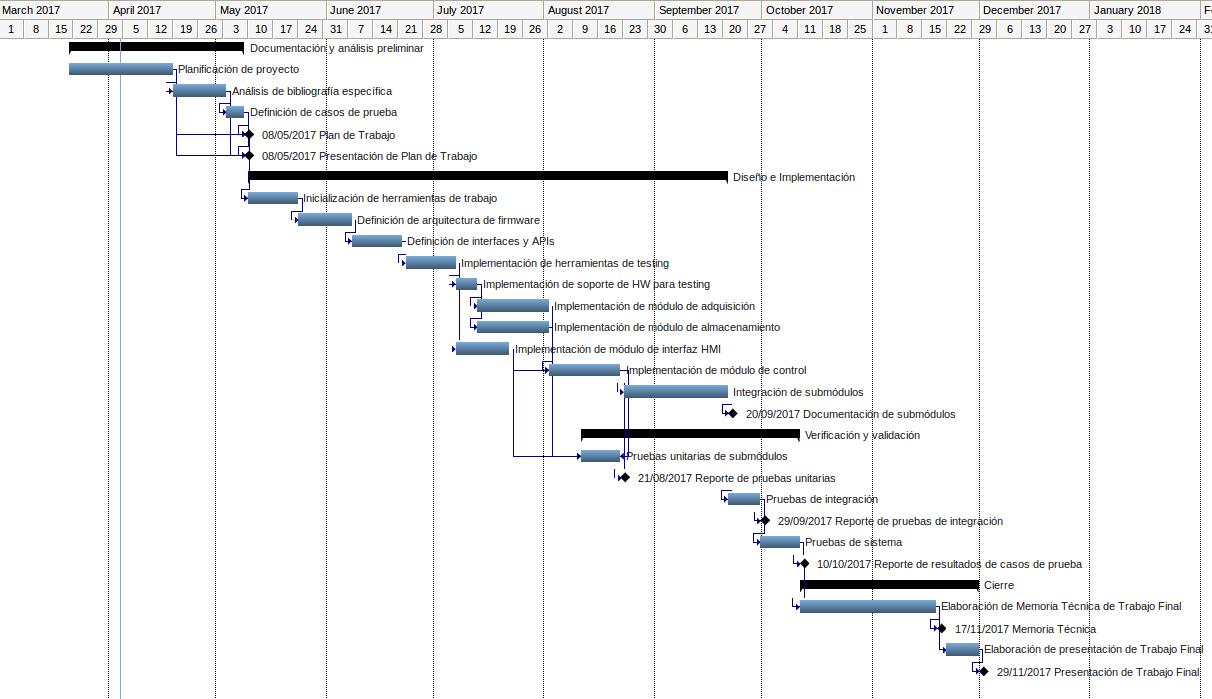
\includegraphics[height=.85\textheight]{./Figuras/Gantt-2.png}
%\caption{Ejemplo de diagrama de Gantt rotado}
%\label{fig:diagGantt}
%\end{figure}
%
%\end{landscape}
%
%\end{consigna}

%\begin{landscape}
\rotatebox{90}{%
\begin{ganttchart}[
	hgrid,
    vgrid={*4{dotted}, *3{red!50}}, %	vgrid,
	x unit=0.12cm,
	y unit chart=0.7cm,
	time slot format=isodate,
	time slot unit=day,
	bar/.append style={fill=blue!30},
	group/.append style={fill=blue!50},
	%link/.style={->, thick}
	]{2023-09-11}{2024-01-24}
	
	\gantttitlecalendar{year, month} \\
			\ganttmilestone{0. Acta de Constitución}{2023-09-11}\\
		\ganttgroup{1 Gestión del Proyecto}{2023-09-11}{2023-10-13} \\
		\ganttbar[name=11]{1.1 Generación de requerimientos}{2023-09-11}{2023-09-15} \\
		\ganttbar[name=12]{1.2 Planificación del proyecto}{2023-09-18}{2023-09-29} \\
		\ganttbar{1.3 Planificación de entregables}{2023-10-02}{2023-10-04} \\
		\ganttbar{1.4 Revisión y ajustes}{2023-10-04}{2023-10-13} \\
			\ganttmilestone{1.5 Proyecto de tesis}{2023-10-13} \\
	
	\ganttgroup{2 Diseño General}{2023-10-16}{2023-11-03} \\
		\ganttbar{2.1 Ajuste al diseño conceptual}{2023-10-16}{2023-10-18} \\
		\ganttbar{2.2 Diagramas de flujo}{2023-10-18}{2023-10-25} \\
		\ganttbar{2.3 Revisión y ajustes de diseño}{2023-10-25}{2023-11-03} \\
	
	\ganttgroup{3 Construcción del hardware}{2023-11-06}{2023-12-15} \\
		\ganttbar{3.1 Selección de componentes}{2023-11-06}{2023-11-10} \\
		\ganttbar{3.2 Diseño de circuitos}{2023-11-13}{2023-11-24} \\
		\ganttbar{3.3 Montaje y soldadura}{2023-11-27}{2023-12-06} \\
		\ganttbar{3.4 Pruebas iniciales}{2023-12-06}{2023-12-15} \\
	
	\ganttgroup{4 Diseño del firmware}{2023-12-18}{2024-01-24} \\
		\ganttbar{4.1 Diseño de arquitectura}{2023-12-18}{2023-12-22} \\
		\ganttbar{4.2 Implementación de MP2,5}{2023-12-25}{2024-01-03} \\
		\ganttbar{4.3 Almacenamiento y comunicación}{2024-01-03}{2024-01-12} \\
		\ganttbar{4.4 Funciones auxiliares}{2024-01-15}{2024-01-24} 
	
	\ganttlink[]{11}{12}
	
\end{ganttchart}
}
\newpage
\rotatebox{90}{%
\begin{ganttchart}[
	hgrid,
%vgrid,
 vgrid={*4{dotted}, *3{red!50}}, %	vgrid,
x unit=0.14cm,
y unit chart=0.7cm,
time slot format=isodate,
time slot unit=day,
bar/.append style={fill=blue!30},
group/.append style={fill=blue!50},
bar/.append style={fill=blue!30, bar label node/.append style={above=3pt}},
%include title in canvas=false,
%inline,
milestone inline label node/.append style={left=5mm}
%link/.style={->, thick}
%link label font=\small\bfseries\color{purple}
link/.style={|-to, line width=0.5pt, blue},
    bar inline label node/.style={
	anchor=east,
	xshift=+4.5cm,
	yshift=0.4cm,
}
]{2024-01-22}{2024-05-28}
	
	\gantttitlecalendar{year, month} \\
	
	\ganttgroup{5 Realización de pruebas}{2024-01-24}{2024-02-21} \\
		\ganttbar[name=51]{5.1 Diseño de casos de prueba}{2024-01-24}{2024-01-31} \\
		\ganttbar[name=52]{5.2 Ejecución de pruebas}{2024-01-31}{2024-02-14} \\
		\ganttbar[name=53]{5.3 Análisis de resultados}{2024-02-14}{2024-02-21} \\
		
	\ganttgroup{6 Ajustes finales}{2024-02-21}{2024-03-06} \\
		\ganttbar[name=61]{6.1 Depuración de errores}{2024-02-21}{2024-02-28} \\
		\ganttbar{6.2 Ajustes de performance}{2024-02-28}{2024-03-06} \\
			\ganttmilestone{6.3 Prototipo funcional}{2024-03-06} \\
		
	\ganttgroup{7 Generación escrito y manuales}{2024-03-06}{2024-05-08} \\
		\ganttbar{7.1 Marco teórico}{2024-03-06}{2024-03-20} \\
		\ganttbar{7.2 Metodología}{2024-03-20}{2024-03-27} \\
		\ganttbar{7.3 Implementación}{2024-03-27}{2024-04-03} \\
		\ganttbar{7.4 Resultados y conclusiones}{2024-04-03}{2024-04-10} \\
		\ganttbar{7.5 Introducción, resumen y otros}{2024-04-10}{2024-04-19} \\
		\ganttbar{7.6 Manual de usuario}{2024-04-22}{2024-04-26} \\
		\ganttbar{7.7 Manual técnico}{2024-04-29}{2024-05-08} \\
			\ganttmilestone{7.8 Manual técnico}{2024-05-08} \\
	
	\ganttgroup{8 Entregas del trabajo final}{2024-05-08}{2024-05-22} \\
		\ganttbar{8.1 Preparación de la presentación}{2024-05-08}{2024-05-22} \\
		\ganttbar{8.2 Presentación del trabajo final}{2024-05-22}{2024-05-22} \\
			\ganttmilestone{8.3 Informe final y presentación}{2024-05-22}
	
	\ganttlink[]{51}{52}
	\ganttlink[]{52}{53}
	\ganttlink[]{53}{61}

\end{ganttchart}
%\end{landscape}
}


% TODO: \usepackage{graphicx} required

%\includegraphics[width=0.9\textwidth, angle=270]{../planner/salida}





%\begin{consigna}{red}
%
%Existen muchos programas y recursos \textit{online} para hacer diagramas de Gantt, entre los cuales destacamos:
%
%\begin{itemize}
%\item Planner
%\item GanttProject
%\item Trello + \textit{plugins}. En el siguiente link hay un tutorial oficial: \\ \url{https://blog.trello.com/es/diagrama-de-gantt-de-un-proyecto}
%\item Creately, herramienta online colaborativa. \\\url{https://creately.com/diagram/example/ieb3p3ml/LaTeX}
%\item Se puede hacer en latex con el paquete \textit{pgfgantt}\\ \url{http://ctan.dcc.uchile.cl/graphics/pgf/contrib/pgfgantt/pgfgantt.pdf}
%\end{itemize}
%
%Pegar acá una captura de pantalla del diagrama de Gantt, cuidando que la letra sea suficientemente grande como para ser legible. 
%Si el diagrama queda demasiado ancho, se puede pegar primero la ``tabla'' del Gantt y luego pegar la parte del diagrama de barras del diagrama de Gantt.
%
%Configurar el software para que en la parte de la tabla muestre los códigos del EDT (WBS).\\
%Configurar el software para que al lado de cada barra muestre el nombre de cada tarea.\\
%Revisar que la fecha de finalización coincida con lo indicado en el Acta Constitutiva.
%
%En la figura \ref{fig:gantt}, se muestra un ejemplo de diagrama de Gantt realizado con el paquete de \textit{pgfgantt}. En la plantilla pueden ver el código que lo genera y usarlo de base para construir el propio.
%
%\begin{figure}[htbp]
%\begin{center}
%\begin{ganttchart}{1}{12}
%  \gantttitle{2020}{12} \\
%  \gantttitlelist{1,...,12}{1} \\
%  \ganttgroup{Group 1}{1}{7} \\
%  \ganttbar{Task 1}{1}{2} \\
%  \ganttlinkedbar{Task 2}{3}{7} \ganttnewline
%  \ganttmilestone{Milestone o hito}{7} \ganttnewline
%  \ganttbar{Final Task}{8}{12}
%  \ganttlink{elem2}{elem3}
%  \ganttlink{elem3}{elem4}
%\end{ganttchart}
%\end{center}
%\caption{Diagrama de Gantt de ejemplo}
%\label{fig:gantt}
%\end{figure}
%
%
%\begin{landscape}
%\begin{figure}[htpb]
%\centering 
%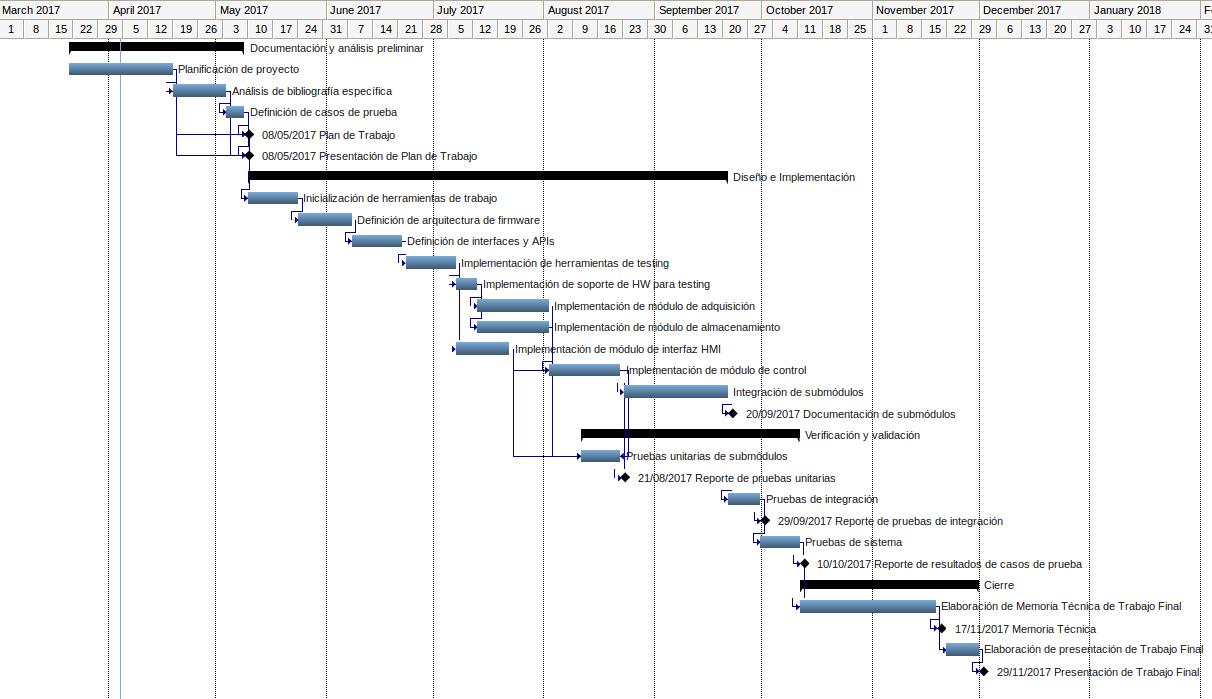
\includegraphics[height=.85\textheight]{./Figuras/Gantt-2.png}
%\caption{Ejemplo de diagrama de Gantt rotado}
%\label{fig:diagGantt}
%\end{figure}
%
%\end{landscape}
%
%\end{consigna}

%\begin{landscape}
\rotatebox{90}{%
\begin{ganttchart}[
	hgrid,
    vgrid={*4{dotted}, *3{red!50}}, %	vgrid,
	x unit=0.12cm,
	y unit chart=0.7cm,
	time slot format=isodate,
	time slot unit=day,
	bar/.append style={fill=blue!30},
	group/.append style={fill=blue!50},
	%link/.style={->, thick}
	]{2023-09-11}{2024-01-24}
	
	\gantttitlecalendar{year, month} \\
			\ganttmilestone{0. Acta de Constitución}{2023-09-11}\\
		\ganttgroup{1 Gestión del Proyecto}{2023-09-11}{2023-10-13} \\
		\ganttbar[name=11]{1.1 Generación de requerimientos}{2023-09-11}{2023-09-15} \\
		\ganttbar[name=12]{1.2 Planificación del proyecto}{2023-09-18}{2023-09-29} \\
		\ganttbar{1.3 Planificación de entregables}{2023-10-02}{2023-10-04} \\
		\ganttbar{1.4 Revisión y ajustes}{2023-10-04}{2023-10-13} \\
			\ganttmilestone{1.5 Proyecto de tesis}{2023-10-13} \\
	
	\ganttgroup{2 Diseño General}{2023-10-16}{2023-11-03} \\
		\ganttbar{2.1 Ajuste al diseño conceptual}{2023-10-16}{2023-10-18} \\
		\ganttbar{2.2 Diagramas de flujo}{2023-10-18}{2023-10-25} \\
		\ganttbar{2.3 Revisión y ajustes de diseño}{2023-10-25}{2023-11-03} \\
	
	\ganttgroup{3 Construcción del hardware}{2023-11-06}{2023-12-15} \\
		\ganttbar{3.1 Selección de componentes}{2023-11-06}{2023-11-10} \\
		\ganttbar{3.2 Diseño de circuitos}{2023-11-13}{2023-11-24} \\
		\ganttbar{3.3 Montaje y soldadura}{2023-11-27}{2023-12-06} \\
		\ganttbar{3.4 Pruebas iniciales}{2023-12-06}{2023-12-15} \\
	
	\ganttgroup{4 Diseño del firmware}{2023-12-18}{2024-01-24} \\
		\ganttbar{4.1 Diseño de arquitectura}{2023-12-18}{2023-12-22} \\
		\ganttbar{4.2 Implementación de MP2,5}{2023-12-25}{2024-01-03} \\
		\ganttbar{4.3 Almacenamiento y comunicación}{2024-01-03}{2024-01-12} \\
		\ganttbar{4.4 Funciones auxiliares}{2024-01-15}{2024-01-24} 
	
	\ganttlink[]{11}{12}
	
\end{ganttchart}
}
\newpage
\rotatebox{90}{%
\begin{ganttchart}[
	hgrid,
%vgrid,
 vgrid={*4{dotted}, *3{red!50}}, %	vgrid,
x unit=0.14cm,
y unit chart=0.7cm,
time slot format=isodate,
time slot unit=day,
bar/.append style={fill=blue!30},
group/.append style={fill=blue!50},
bar/.append style={fill=blue!30, bar label node/.append style={above=3pt}},
%include title in canvas=false,
%inline,
milestone inline label node/.append style={left=5mm}
%link/.style={->, thick}
%link label font=\small\bfseries\color{purple}
link/.style={|-to, line width=0.5pt, blue},
    bar inline label node/.style={
	anchor=east,
	xshift=+4.5cm,
	yshift=0.4cm,
}
]{2024-01-22}{2024-05-28}
	
	\gantttitlecalendar{year, month} \\
	
	\ganttgroup{5 Realización de pruebas}{2024-01-24}{2024-02-21} \\
		\ganttbar[name=51]{5.1 Diseño de casos de prueba}{2024-01-24}{2024-01-31} \\
		\ganttbar[name=52]{5.2 Ejecución de pruebas}{2024-01-31}{2024-02-14} \\
		\ganttbar[name=53]{5.3 Análisis de resultados}{2024-02-14}{2024-02-21} \\
		
	\ganttgroup{6 Ajustes finales}{2024-02-21}{2024-03-06} \\
		\ganttbar[name=61]{6.1 Depuración de errores}{2024-02-21}{2024-02-28} \\
		\ganttbar{6.2 Ajustes de performance}{2024-02-28}{2024-03-06} \\
			\ganttmilestone{6.3 Prototipo funcional}{2024-03-06} \\
		
	\ganttgroup{7 Generación escrito y manuales}{2024-03-06}{2024-05-08} \\
		\ganttbar{7.1 Marco teórico}{2024-03-06}{2024-03-20} \\
		\ganttbar{7.2 Metodología}{2024-03-20}{2024-03-27} \\
		\ganttbar{7.3 Implementación}{2024-03-27}{2024-04-03} \\
		\ganttbar{7.4 Resultados y conclusiones}{2024-04-03}{2024-04-10} \\
		\ganttbar{7.5 Introducción, resumen y otros}{2024-04-10}{2024-04-19} \\
		\ganttbar{7.6 Manual de usuario}{2024-04-22}{2024-04-26} \\
		\ganttbar{7.7 Manual técnico}{2024-04-29}{2024-05-08} \\
			\ganttmilestone{7.8 Manual técnico}{2024-05-08} \\
	
	\ganttgroup{8 Entregas del trabajo final}{2024-05-08}{2024-05-22} \\
		\ganttbar{8.1 Preparación de la presentación}{2024-05-08}{2024-05-22} \\
		\ganttbar{8.2 Presentación del trabajo final}{2024-05-22}{2024-05-22} \\
			\ganttmilestone{8.3 Informe final y presentación}{2024-05-22}
	
	\ganttlink[]{51}{52}
	\ganttlink[]{52}{53}
	\ganttlink[]{53}{61}

\end{ganttchart}
%\end{landscape}
}


% TODO: \usepackage{graphicx} required

%\includegraphics[width=0.9\textwidth, angle=270]{../planner/salida}




%\end{landscape}

\section{12. Presupuesto detallado del proyecto}
\label{sec:presupuesto}
%!TEX root = DisenoProyecto_LuisGomez.tex
%\begin{consigna}{red}
%Si el proyecto es complejo entonces separarlo en partes:
%\begin{itemize}
%	\item Un total global, indicando el subtotal acumulado por cada una de las áreas.
%	\item El desglose detallado del subtotal de cada una de las áreas.
%\end{itemize}
%
%IMPORTANTE: No olvidarse de considerar los COSTOS INDIRECTOS.
%
%\end{consigna}

En el cuadro \ref{tab:presupuesto} se ofrece un desglose de los costos asociados a la presente tesis, todos presentados en dólares estadounidenses (USD). Los costos directos se dividen en categorías: mano de obra y honorarios (\$6.500 USD), materiales y suministros (\$888 USD), viajes y desplazamientos (\$480 USD), equipos y maquinaria (\$300 USD), y otros costos directos asociados a imprevistos (\$1.000 USD), sumando un subtotal de \$8,428 USD. Se incluyen también los costos indirectos, que comprenden arriendo y servicios públicos, con un subtotal de \$1.800 USD. El costo total estimado del proyecto es de \$10.228 USD. 

\begin{table}[htpb]
\centering
\caption{Costos del proyecto de tesis.}
\label{tab:presupuesto}
\small
\begin{tabularx}{\linewidth}{@{}|X|c|r|r|@{}}
\hline
\rowcolor[HTML]{C0C0C0} 
\multicolumn{4}{|c|}{\cellcolor[HTML]{C0C0C0}COSTOS DIRECTOS} \\ \hline
\rowcolor[HTML]{C0C0C0} 
 &
  \multicolumn{1}{c|}{\cellcolor[HTML]{C0C0C0}Cantidad} &
  \multicolumn{1}{c|}{\cellcolor[HTML]{C0C0C0}Valor unitario} &
  \multicolumn{1}{c|}{\cellcolor[HTML]{C0C0C0}Valor total} \\ 
\rowcolor[HTML]{C0C0C0} Descripción  &
  \multicolumn{1}{c|}{\cellcolor[HTML]{C0C0C0}} &
  \multicolumn{1}{c|}{\cellcolor[HTML]{C0C0C0} \$ USD} &
  \multicolumn{1}{c|}{\cellcolor[HTML]{C0C0C0} \$ USD} \\ \hline
  
\multicolumn{4}{|c|}{\textbf{MANO DE OBRA, HONORARIOS }}\\ \hline
Gestión del Proyecto		& \multicolumn{1}{c|}{	100	} & \multicolumn{1}{c|}{	10	} &  \multicolumn{1}{c|}{	1.000	} \\ \hline
Diseño General				& \multicolumn{1}{c|}{	60	} & \multicolumn{1}{c|}{	10	} &  \multicolumn{1}{c|}{	600	} \\ \hline
Construcción del hardware	& \multicolumn{1}{c|}{	120	} & \multicolumn{1}{c|}{	10	} &  \multicolumn{1}{c|}{	1.200	} \\ \hline
Diseño del firmware			& \multicolumn{1}{c|}{	110	} & \multicolumn{1}{c|}{	10	} &  \multicolumn{1}{c|}{	1.100	} \\ \hline
Realización de pruebas		& \multicolumn{1}{c|}{	120	} & \multicolumn{1}{c|}{	10	} &  \multicolumn{1}{c|}{	1.200	} \\ \hline
Ajustes finales				& \multicolumn{1}{c|}{	40	} & \multicolumn{1}{c|}{	10	} &  \multicolumn{1}{c|}{	400	} \\ \hline
Generación escrito de memoria y manuales	& \multicolumn{1}{c|}{	180	} & \multicolumn{1}{c|}{	10	} &  \multicolumn{1}{c|}{	1800	} \\ \hline
Entregas del trabajo final	& \multicolumn{1}{c|}{	40	} & \multicolumn{1}{c|}{	10	} &  \multicolumn{1}{c|}{	400	} \\ \hline

\multicolumn{4}{|c|}{\textbf{MATERIALES Y SUMINISTROS}}\\ \hline
Placas de desarrollo 	& \multicolumn{1}{c|}{	4	} & \multicolumn{1}{c|}{	50	} &  \multicolumn{1}{c|}{	200	} \\ \hline
Reloj de tiempo real 	& \multicolumn{1}{c|}{	4	} & \multicolumn{1}{c|}{	2	} &  \multicolumn{1}{c|}{	8	} \\ \hline
Placa comunicación		& \multicolumn{1}{c|}{	4	} & \multicolumn{1}{c|}{	10	} &  \multicolumn{1}{c|}{	40	} \\ \hline
Memora flash			& \multicolumn{1}{c|}{	4	} & \multicolumn{1}{c|}{	5	} &  \multicolumn{1}{c|}{	20	} \\ \hline
Fuente poder			& \multicolumn{1}{c|}{	4	} & \multicolumn{1}{c|}{	5	} &  \multicolumn{1}{c|}{	20	} \\ \hline
Gabinete				& \multicolumn{1}{c|}{	4	} & \multicolumn{1}{c|}{	10	} &  \multicolumn{1}{c|}{	40	} \\ \hline
Batería					& \multicolumn{1}{c|}{	4	} & \multicolumn{1}{c|}{	10	} &  \multicolumn{1}{c|}{	40	} \\ \hline
Sensor MP2.5			& \multicolumn{1}{c|}{	16	} & \multicolumn{1}{c|}{	30	} &  \multicolumn{1}{c|}{	480	} \\ \hline
Modem comunicación		& \multicolumn{1}{c|}{	1	} & \multicolumn{1}{c|}{	100	} &  \multicolumn{1}{c|}{	100	} \\ \hline


\multicolumn{4}{|c|}{\textbf{VIAJES Y DESPLAZAMIENTOS}}\\ \hline
Transporte terreno y reuniones	& \multicolumn{1}{c|}{	2	} & \multicolumn{1}{c|}{	100	} &  \multicolumn{1}{c|}{	200	} \\ \hline
Alojamiento terreno 			& \multicolumn{1}{c|}{	4	} & \multicolumn{1}{c|}{	50	} &  \multicolumn{1}{c|}{	200	} \\ \hline
Alimentación					& \multicolumn{1}{c|}{	8	} & \multicolumn{1}{c|}{	10	} &  \multicolumn{1}{c|}{	80	} \\ \hline

\multicolumn{4}{|c|}{\textbf{EQUIPOS Y MAQUINARIA}}\\ \hline
Uso y compra de equipamiento& \multicolumn{1}{c|}{	3	} & \multicolumn{1}{c|}{	100	} &  \multicolumn{1}{c|}{	300	} \\ \hline

\multicolumn{4}{|c|}{\textbf{OTROS COSTOS DIRECTOS}}\\ \hline
Imprevistos	($\sim$10\% del total del  proyecto)				& \multicolumn{1}{c|}{	1	} & \multicolumn{1}{c|}{	1.000	} &  \multicolumn{1}{c|}{	1.000	} \\ \hline

\multicolumn{3}{|c|}{SUBTOTAL COSTOS DIRECTOS} & \multicolumn{1}{c|}{ 8.428 } \\ \hline

\rowcolor[HTML]{C0C0C0} 
\multicolumn{4}{|c|}{\cellcolor[HTML]{C0C0C0}COSTOS INDIRECTOS} \\ \hline
\rowcolor[HTML]{C0C0C0} 
 &
  \multicolumn{1}{c|}{\cellcolor[HTML]{C0C0C0}Cantidad} &
  \multicolumn{1}{c|}{\cellcolor[HTML]{C0C0C0}Valor unitario} &
  \multicolumn{1}{c|}{\cellcolor[HTML]{C0C0C0}Valor total} \\  
\rowcolor[HTML]{C0C0C0} Descripción  &
\multicolumn{1}{c|}{\cellcolor[HTML]{C0C0C0}} &
\multicolumn{1}{c|}{\cellcolor[HTML]{C0C0C0} \$ USD} &
\multicolumn{1}{c|}{\cellcolor[HTML]{C0C0C0} \$ USD} \\ \hline
Arriendo parcial espacio	& \multicolumn{1}{c|}{	8	} & \multicolumn{1}{c|}{	100	} &  \multicolumn{1}{c|}{	800	} \\ \hline
Luz, agua, comunicación y calefacción	& \multicolumn{1}{c|}{	10	} & \multicolumn{1}{c|}{	100	} &  \multicolumn{1}{c|}{	1.000	} \\ \hline

\multicolumn{3}{|c|}{SUBTOTAL COSTOS INDIRECTOS} &
  \multicolumn{1}{c|}{1.800 } \\ \hline
\rowcolor[HTML]{C0C0C0}
\multicolumn{3}{|c|}{TOTAL} &
\multicolumn{1}{c|}{10.228 }
   \\ \hline
\end{tabularx}%
\end{table}


\section{13. Gestión de riesgos}
\label{sec:riesgos}
%!TEX root = DisenoProyecto_LuisGomez.tex

\definecolor{GreenColor}{rgb}{0.0, 1.0, 0.0} % Definir color verde
\definecolor{LightRed}{rgb}{1.0, 0.6, 0.6} % Definir color rojo suave
\definecolor{RedColor}{rgb}{1.0, 0.0, 0.0} % Definir color rojo
\definecolor{GreenColor}{HTML}{00FF00}
\definecolor{LightRed}{HTML}{FF6666}
\definecolor{RedColor}{HTML}{FF0000}

\newcommand{\colorcell}[1]{%
	\ifnum#1<10 \cellcolor{GreenColor}%
	\else\ifnum#1<20 \cellcolor{GreenColor!50}%
	\else\ifnum#1<30 \cellcolor{GreenColor!30}%
	\else\ifnum#1<40 \cellcolor{LightRed}%
	\else\ifnum#1<50 \cellcolor{RedColor!50}%
	\else\ifnum#1<60 \cellcolor{RedColor!60}%
	\else\ifnum#1<70 \cellcolor{RedColor!70}%
	\else\ifnum#1<80 \cellcolor{RedColor!80}%
	\else\ifnum#1<90 \cellcolor{RedColor!90}%
	\else \cellcolor{RedColor}%
	\fi\fi\fi\fi\fi\fi\fi\fi\fi
	#1%
}


Los riesgos se clasificarán mediante una escala lineal que opera en un rango de \(1\) a \(10\), fundamentándose en las características distintivas que se describen a continuación:

\begin{description}
	\item[Severidad (S):] Se asignará un valor numérico más elevado a aquellos riesgos que presenten un mayor nivel de severidad.
	\item[Probabilidad de Ocurrencia (O):] Los riesgos con una mayor probabilidad de ocurrencia recibirán un número más alto.
\end{description}

El número de prioridad de riesgo (RPN) se derivará mediante el producto de la Severidad (S) y la Probabilidad de Ocurrencia (O), siguiendo la fórmula:

\[ S \times O = RPN \]

Como resultado de la fórmula anterior, el \(0\) simboliza la prioridad más baja y el \(100\) la más alta, como se muestra en la tabla \ref{tab:rpn}. De forma arbitraria, se ha definido el \(30\) como el nivel crítico tolerable de RPN, por debajo del cual (valores menores a 30), no es imperativo implementar medidas para eliminar, mitigar o transferir el riesgo.





\begin{table}[htbp]
	\caption{Escala de número de prioridad del riesgo (RPN)}
	\label{tab:rpn}
	\centering
	\begin{tabular}{lc}
		\hline
		\textbf{Descriptor} & \textbf{RPN} \\
		\hline
		BAJO & \cellcolor{GreenColor}0-9 \\
		ACEPTABLE & \cellcolor{GreenColor!50}10-19 \\
		TOLERABLE & \cellcolor{GreenColor!30}20-29 \\
		\hline
		CRÍTICO & \cellcolor{LightRed}30-40 \\
		PELIGROSO & \cellcolor{RedColor!50}40-50 \\
		PELIGROSO  & \cellcolor{RedColor!60}50-60 \\	
		PELIGROSO  & \cellcolor{RedColor!70}60-70 \\
		MUY ALTO & \cellcolor{RedColor!80}70-80 \\
		MUY ALTO & \cellcolor{RedColor!90}80-90 \\
		ALTISIMO & \cellcolor{RedColor}90-100 \\
		\hline
	\end{tabular}
\end{table}

\subsection{ Identificación de los riesgos y estimación de sus consecuencias:}
	\begin{description}
		
	\item[Riesgo 1:]\textbf{Mal funcionamiento de los sensores de MP2,5}
		\begin{itemize}
			\item \textbf{Severidad (S): 9} \\
			Justificación: un mal funcionamiento en los sensores de MP2,5 podría generar mediciones imprecisas en la concentración de partículas. Estas mediciones erróneas pueden conducir a decisiones inadecuadas en relación con la gestión de la calidad del aire, con potenciales implicancias en la salud pública.
			
			\item \textbf{Probabilidad de ocurrencia (O): 7} \\
			Justificación: la utilización de sensores de bajo costo aumenta significativamente la probabilidad de fallos y, por ende, de mediciones incorrectas.
			\item \textbf{Número de prioridad de riesgo (RPN): 63} \\
		\end{itemize}


    \item[Riesgo 2:] \textbf{Autoridades no aceptan como válidas las mediciones realizadas con sensores de MP2,5 de bajo costo}   	 
		\begin{itemize}
			\item \textbf{Severidad (S): 7}\\
			Justificación: los sensores ópticos no están actualmente reconocidos por la Agencia de Protección Ambiental (EPA) como una técnica analítica estándar para la medición de MP2,5.
			
			\item \textbf{Probabilidad de ocurrencia (O): 8} \\
			Justificación: muchos países mantienen los métodos gravimétricos como una técnica analítica normada para la medición de las concentraciones MP2,5 atmosférico.
			\item \textbf{Número de prioridad de riesgo (RPN): 56} \\
		\end{itemize}  
 
	
	\item[Riesgo 3:] \textbf{\underline{Fallo en la transmisión de datos en línea}}
	\begin{itemize}
		\item \textbf{Severidad (S): 6} \\
		Justificación: un fallo en la transmisión de datos puede provocar una pérdida de información momentánea en el servidor central encargado de administrar los datos. Esta situación podría ocasionar la pérdida de la oportunidad de tomar decisiones informadas y a tiempo respecto a la calidad del aire o del funcionamiento del instrumento.
		
		\item \textbf{Probabilidad de ocurrencia (O): 5} \\
		Justificación: es común experimentar pérdidas en la conexión inalámbrica debido a diversas fallas como interrupciones del servicio de internet, cortes de suministro eléctrico, impago de la cuenta de internet, entre otros. 
		 
		\item \textbf{Número de prioridad de riesgo (RPN): 30} \\
	\end{itemize}

	
	\item[Riesgo 4:] \underline{\textbf{Interrupción de energía en el sistema}}
	\begin{itemize}
		\item \textbf{Severidad (S): 8} \\
		Justificación: una interrupción en el suministro de energía puede llevar a pérdidas de medición durante periodos de tiempo determinados, afectando la continuidad y la integridad de los datos registrados.
		
		\item \textbf{Probabilidad de ocurrencia (O): 4} \\
		Justificación: aunque la posibilidad de interrupciones en el suministro de energía es real, en entornos urbanos la frecuencia de estos eventos tiende a ser baja, debido a la infraestructura y los respaldos energéticos existentes.
		
		\item \textbf{Número de prioridad de riesgo (RPN): 32} \\

	\end{itemize}

	
	\item[Riesgo 5:] \underline{\textbf{Manipulación o actos vandalismo en las estaciones de monitoreo}}
	\begin{itemize}
		\item \textbf{Severidad (S): 8} \\
		Justificación: la manipulación indebida o actos de vandalismo dirigidos a las estaciones de monitoreo podrían comprometer la calidad y confiabilidad de los datos recabados, afectando la integridad del sistema de monitoreo y, por ende, la validez de los análisis subsiguientes.
		
		\item \textbf{Probabilidad de ocurrencia (O): 3} \\
		Justificación: a pesar de que las estaciones se localizan en zonas consideradas seguras y sujetas a vigilancia, la posibilidad de incidencias de vandalismo o manipulación indebida persiste, aunque a un nivel reducido.
		
		\item \textbf{Número de prioridad de riesgo (RPN): 24} \\
	\end{itemize}

	
\item[Riesgo 6:] \underline{\textbf{Pérdida de sincronización del Reloj de Tiempo Real (RTC)}}
\begin{itemize}
	\item \textbf{Severidad (S): 7} \\
	Justificación: la pérdida de sincronización del reloj de tiempo real (RTC) conlleva que los datos adquiridos pierdan exactitud en sus etiquetas temporales. Esto impide discernir el instante de cada medición, lo cual puede degradar significativamente la utilidad y relevancia de los datos recopilados, afectar calibraciones y, en casos extremos, volver los datos inservibles.
	
	\item \textbf{Probabilidad de ocurrencia (O): 3} \\
	Justificación: los RTC actuales, como el DS3231, son robustos y mantienen una precisión considerable, con desviaciones menores al minuto a lo largo de un año, lo que hace que la probabilidad de desincronización sea relativamente baja, pero existente.
	
	\item \textbf{Número de prioridad de riesgo (RPN): 21} \\
\end{itemize}




\end{description}


\subsection{Plan de mitigación de los riesgos}

Se implementarán estrategias de mitigación para los riesgos que presenten Número de prioridad de riesgo (\textbf{RPN}) superiores a 25. Dichas estrategias estarán detalladas a continuación y afectarán directamente tanto a la severidad (\textbf{S}) como a la probabilidad de ocurrencia (\textbf{\textit{O}}) de los riesgos identificados. La severidad y probabilidad de ocurrencia modificadas tras la implementación del plan de mitigación se denotarán como \textbf{S*} y \textbf{O*}, respectivamente. Estas modificaciones podrán dar como resultado un nuevo \textbf{RPN*}, el que deberá, en la medida de lo posible, ajustarse al criterio de aceptabilidad previamente establecido, es decir, ser inferior a 25.

\begin{description}
	\item[Riesgo 1:]\textbf{Mal funcionamiento de los sensores de MP2,5}
		\begin{itemize}
			\item \textbf{Plan de mitigación:} para cada equipo, se incorporarán tres sensores, y, en caso de fallo de alguno de ellos, se remitirá un código de falla al administrador.
			\item \textbf{Severidad (S*): 9} \\
			Efecto de la medida: A pesar de las medidas de mitigación, la severidad del efecto en caso de fallo del sensor se mantiene.
			\item \textbf{Probabilidad de ocurrencia (O*): 2} \\
			Efecto de la medida: se anticipa una reducción en la probabilidad de fallo integral del instrumento. La inclusión de múltiples sensores permite que, en caso de fallo de uno, los demás continúen operativos, permitiendo el aviso inmediato al administrador mediante el envío de un código de falla, lo que previene interrupciones totales en la medición.
			\item \textbf{Número de prioridad de riesgo (RPN*): 18} 
		\end{itemize}
	


    \item[Riesgo 2:] \textbf{Autoridades no aceptan como válidas las mediciones realizadas con sensores de MP2,5 de bajo costo}   	 
		\begin{itemize}
			
			\item \textbf{Plan de mitigación:} realización de pruebas de calibración con sensores que cuenten con la aprobación EPA o su equivalencia para MP2,5. Mostrar a las autoridades, mediante estudios y pruebas de calibración,que este tipo de instrumentos pueden ser puntos de medición complementarios, que aportan mayor densidad  de muestreo a las actuales redes de monitoreo de calidad del aire. Y mostrar la robustez del sistema estadístico planteado y el bajo costo que implica esta tecnología.   
			\item \textbf{Severidad (S*): 6} \\
			Efecto de la medida: sobre la base los antecedentes aportados por la calibración y los costos comparados de esta tecnología, los servicios ambientales y gobiernos locales acepten emplear este tipo de tecnologías como métodos alternativos y complementarios para sus monitoreos de la calidad del aire. cabe mencionar que esta tecnología presenta incertidumbre de operación en un rango amplio de concentraciones. Por ejemplo en concentraciones muy altas por lo que la severidad no desaparecerá del todo.
	
			\item \textbf{Probabilidad de ocurrencia (O*): 4} \\
			Efecto de la medida: en actualidad, en base a resultados de investigaciones y pruebas pilotos, algunos servicios ambientales y gobiernos locales se están abriendo a emplear metodologías de bajo costo para ampliar sus redes de monitoreo o tener primeras aproximaciones de las calidad del aire en centros urbanos.
			\item \textbf{Número de prioridad de riesgo (RPN*): 24} 
			\end{itemize}	
			
		\item[Riesgo 3:] \textbf{\underline{Fallo en la transmisión de datos en línea}}
	\begin{itemize}
			\item \textbf{Plan de mitigación:} se sugiere equipar el instrumento con un sistema de almacenamiento local de datos, lo que permitiría recuperar los datos ausentes en caso de una desconexión.
			
			\item \textbf{Severidad (S*): 2} \\
			Efecto de la medida: dado que los datos pueden ser recuperados mediante el almacenamiento local de datos, la severidad del problema se reduce significativamente.
			
			\item \textbf{Probabilidad de ocurrencia (O*): 5} \\
			Efecto de la medida: no se anticipan cambios en la frecuencia de interrupciones, ya que se continuará utilizando el mismo sistema de conexión.
			
			\item \textbf{Número de prioridad de riesgo (RPN*): 10}
	\end{itemize}

			\item[Riesgo 4:] \textbf{\underline{Interrupción de energía en el sistema}}
	\begin{itemize}
			\item \textbf{Plan de mitigación:} se implementará un sistema de respaldo energético, como baterías, para asegurar una autonomía limitada en caso de cortes de energía. Asimismo, se planea habilitar opciones de modo de bajo consumo para el instrumento, durante los cortes, pueda apagar componentes de transmisión de datos o reducir la frecuencia de muestreo, por ejemplo.
			
			\item \textbf{Severidad (S*): 6} \\
			Efecto de la medida: la implementación de un respaldo energético permitirá mantener el instrumento en funcionamiento durante cortes de energía, probablemente por algunos minutos adicionales.
			
			\item \textbf{Probabilidad de ocurrencia (O*): 2} \\
			Efecto de la medida: Se anticipa que los cortes breves de energía, comunes en algunos sistemas eléctricos, no afectarán el funcionamiento normal del instrumento. Sin embargo, los cortes prolongados de energía pueden seguir siendo problemáticos.
			
			\item \textbf{Número de prioridad de riesgo (RPN*): 12}
	\end{itemize}

 
\end{description}




\subsection{Gestión de riesgos}


A partir de los resultados adquiridos del análisis de riesgo y su respectiva gestión, se exhibe el Cuadro~\ref{tab:gestionriesgo}. En él se sintetizan, tanto de forma numérica como gráfica, los impactos de las estrategias de mitigación en el \textbf{RPN}. El Cuadro~\ref{tab:gestionriesgo} evidencia que las estrategias de gestión propuestas consiguen reducir el riesgo a niveles aceptables, conforme a los criterios previamente establecidos.


	
	\begin{table}[htpb]
		
		\caption{Resumen de la gestión del riesgos con el resultado de las medidas de mitigación.}
		\label{tab:gestionriesgo}
		\centering
		\begin{tabularx}{\linewidth}{|X|c|c|c|c|c|c|}
			\hline
			\rowcolor[HTML]{C0C0C0} 
			Riesgo & S & O & RPN & S* & O* & RPN* \\ \hline
			Mal funcionamiento de los sensores & 9  & 8  & \colorcell{72}    & 5  & 4  & \colorcell{20}    \\ \hline
			Autoridades no aceptan mediciones  & 7  & 8  & \colorcell{56}    & 4  & 4  & \colorcell{16}    \\ \hline
			Fallo en la transmisión de datos   & 6  & 5  & \colorcell{30}    & 3  & 2  & \colorcell{6}     \\ \hline
			Interrupción de energía            & 8  & 4  & \colorcell{32}    & 4  & 2  & \colorcell{8}     \\ \hline
			Manipulación o actos vandalismo    & 8  & 3  & \colorcell{24}    & -  & -  & -     \\ \hline
			Pérdida de sincronización del RTC  & 7  & 3  & \colorcell{21}    & -  & -  & -     \\ \hline
		\end{tabularx}%
	\end{table}
	
	
	\textbf{Nota: }los valores marcados con (\textbf{*}) en la tabla corresponden luego de haber aplicado la mitigación.
	


%\begin{consigna}{red}
%a) Identificación de los riesgos (al menos cinco) y estimación de sus consecuencias:
% 
%Riesgo 1: detallar el riesgo (riesgo es algo que si ocurre altera los planes previstos de forma negativa)
%\begin{itemize}
%	\item Severidad (S): mientras más severo, más alto es el número (usar números del 1 al 10).\\
%	Justificar el motivo por el cual se asigna determinado número de severidad (S).
%	\item Probabilidad de ocurrencia (O): mientras más probable, más alto es el número (usar del 1 al 10).\\
%	Justificar el motivo por el cual se asigna determinado número de (O). 
%\end{itemize}   
%
%Riesgo 2:
%\begin{itemize}
%	\item Severidad (S): 
%	\item Ocurrencia (O):
%\end{itemize}
%
%Riesgo 3:
%\begin{itemize}
%	\item Severidad (S): 
%	\item Ocurrencia (O):
%\end{itemize}
%
%
%b) Tabla de gestión de riesgos:      (El RPN se calcula como RPN=SxO)
%
%\begin{table}[htpb]
%\centering
%\begin{tabularx}{\linewidth}{@{}|X|c|c|c|c|c|c|@{}}
%\hline
%\rowcolor[HTML]{C0C0C0} 
%Riesgo & S & O & RPN & S* & O* & RPN* \\ \hline
%       &   &   &     &    &    &      \\ \hline
%       &   &   &     &    &    &      \\ \hline
%       &   &   &     &    &    &      \\ \hline
%       &   &   &     &    &    &      \\ \hline
%       &   &   &     &    &    &      \\ \hline
%\end{tabularx}%
%\end{table}
%
%Criterio adoptado: 
%Se tomarán medidas de mitigación en los riesgos cuyos números de RPN sean mayores a...
%
%Nota: los valores marcados con (*) en la tabla corresponden luego de haber aplicado la mitigación.
%
%c) Plan de mitigación de los riesgos que originalmente excedían el RPN máximo establecido:
% 
%Riesgo 1: plan de mitigación (si por el RPN fuera necesario elaborar un plan de mitigación).
%  Nueva asignación de S y O, con su respectiva justificación:
%  - Severidad (S): mientras más severo, más alto es el número (usar números del 1 al 10).
%          Justificar el motivo por el cual se asigna determinado número de severidad (S).
%  - Probabilidad de ocurrencia (O): mientras más probable, más alto es el número (usar del 1 al 10).
%          Justificar el motivo por el cual se asigna determinado número de (O).
%
%Riesgo 2: plan de mitigación (si por el RPN fuera necesario elaborar un plan de mitigación).
% 
%Riesgo 3: plan de mitigación (si por el RPN fuera necesario elaborar un plan de mitigación).
%
%\end{consigna}

\section{14. Gestión de la calidad}
\label{sec:calidad}
%!TEX root = DisenoProyecto_LuisGomez.tex
%\begin{consigna}{red}
%Elija al menos diez requerientos que a su criterio sean los más importantes/críticos/que aportan más valor y para cada uno de ellos indique las acciones de verificación y validación que permitan asegurar su cumplimiento.
%
%\begin{itemize} 
%\item Req \#1: copiar acá el requerimiento.
%
%\begin{itemize}
%	\item Verificación para confirmar si se cumplió con lo requerido antes de mostrar el sistema al cliente. Detallar 
%	\item Validación con el cliente para confirmar que está de acuerdo en que se cumplió con lo requerido. Detallar  
%\end{itemize}
%
%\end{itemize}
%
%Tener en cuenta que en este contexto se pueden mencionar simulaciones, cálculos, revisión de hojas de datos, consulta con expertos, mediciones, etc.  Las acciones de verificación suelen considerar al entregable como ``caja blanca'', es decir se conoce en profundidad su funcionamiento interno.  En cambio, las acciones de validación suelen considerar al entregable como ``caja negra'', es decir, que no se conocen los detalles de su funcionamiento interno.
%
%\end{consigna}






Elija al menos diez requerimientos que a su criterio sean los más importantes/críticos/que aportan más valor y para cada uno de ellos indique las acciones de verificación y validación que permitan asegurar su cumplimiento.

\begin{itemize} 
\item Req \#1: Funcionamiento correcto y preciso de los sensores para medir la calidad del agua.

\begin{itemize}
	\item Verificación: Realizar pruebas y simulaciones para asegurarse de que los sensores miden con precisión los parámetros de la calidad del agua. Consultar con expertos y revisar las hojas de datos de los sensores para confirmar la precisión y fiabilidad de las mediciones.
	\item Validación: Realizar mediciones en campo y comparar los resultados obtenidos con mediciones estándar y aceptadas para asegurar la exactitud y conformidad de los sensores en condiciones reales.
\end{itemize}

\item Req \#2: Transmisión de datos segura y sin fallos desde los sensores hasta la base de datos.

\begin{itemize}
	\item Verificación: Probar la transmisión de datos en diferentes condiciones y con diferentes volúmenes de datos para asegurar la robustez y fiabilidad del sistema de transmisión.
	\item Validación: Confirmar con el cliente mediante pruebas de transmisión de datos en tiempo real para asegurar que los datos se reciben correctamente y en tiempo.
\end{itemize}

\item Req \#3: Sistema de alimentación energética ininterrumpida y fiable.

\begin{itemize}
	\item Verificación: Realizar pruebas de estrés al sistema de alimentación para asegurar su capacidad de mantenerse operativo en situaciones de corte de energía.
	\item Validación: Demostrar al cliente mediante pruebas de funcionamiento prolongado que el sistema puede operar de forma continua sin interrupciones debidas a fallos de energía.
\end{itemize}



\end{itemize}



\section{15. Procesos de cierre}    
\label{sec:cierre}
%!TEX root = DisenoProyecto_LuisGomez.tex
%\begin{consigna}{red}
%Establecer las pautas de trabajo para realizar una reunión final de evaluación del proyecto, tal que contemple las siguientes actividades:
%
%\begin{itemize}
%	\item Pautas de trabajo que se seguirán para analizar si se respetó el Plan de Proyecto original:
%	 - Indicar quién se ocupará de hacer esto y cuál será el procedimiento a aplicar. 
%	\item Identificación de las técnicas y procedimientos útiles e inútiles que se emplearon, y los problemas que surgieron y cómo se solucionaron:
%	 - Indicar quién se ocupará de hacer esto y cuál será el procedimiento para dejar registro.
%	\item Indicar quién organizará el acto de agradecimiento a todos los interesados, y en especial al equipo de trabajo y colaboradores:
%	  - Indicar esto y quién financiará los gastos correspondientes.
%\end{itemize}
%
%\end{consigna}


Se realizará una reunión final para evaluar el proyecto, analizar el cumplimiento del Plan de Proyecto original, identificar técnicas y procedimientos útiles, abordar los problemas surgidos y organizar un acto de agradecimiento para todos los participantes.

\subsection{Pautas de trabajo para analizar el respeto al Plan de Proyecto original}
\begin{itemize}
	\item \textbf{Responsable:} El Jefe de Proyecto.
	\item \textbf{Procedimiento:} Comparar los resultados obtenidos con los objetivos establecidos en el Plan de Proyecto original, documentar desviaciones y analizar sus causas.
	\item \textbf{Registro:} Documento final de análisis comparativo.
\end{itemize}

\subsection{Identificación de técnicas y procedimientos y solución de problemas}
\begin{itemize}
	\item \textbf{Responsable:} El Jefe de Proyecto.
	\item \textbf{Procedimiento:} Realizar reuniones de retrospectiva para discutir y documentar las lecciones aprendidas y los problemas surgidos.
	\item \textbf{Registro:} Documento de "Lecciones Aprendidas".
\end{itemize}

\subsection{Acto de agradecimiento}
\begin{itemize}
	\item \textbf{Organizador:} El Jefe de Proyecto.
	\item \textbf{Procedimiento:} Ceremonia de agradecimiento y entrega de certificados de reconocimiento.
\end{itemize}

\subsection{Cronograma de cierre}
\begin{itemize}
	\item \textbf{Reunión de Evaluación del Proyecto:} [Fecha a determinar]
	\item \textbf{Entrega de Documento de Análisis Comparativo:} [Fecha a determinar]
	\item \textbf{Entrega de Documento de Lecciones Aprendidas:} [Fecha a determinar]
	\item \textbf{Ceremonia de Agradecimiento:} [Fecha a determinar]
\end{itemize}

\subsection*{Participantes}
Todos los miembros del equipo de proyecto, colaboradores, interesados y patrocinadores están invitados a participar en las actividades de cierre.



\end{document}
